%
%

\documentclass[11pt,a4paper,oneside]{book}

\usepackage[spanish]{babel}
%-------------------------------------------------------------------
% Esto es para poder escribir acentos directamente:
\usepackage[utf8]{inputenc}
\usepackage[T1]{fontenc}
%-----------------------------------------------------------------------
% para uso en modo matamático
\usepackage{amssymb}
\usepackage{amsthm}
\usepackage{amsmath}

\usepackage{hyperref}   



\usepackage{pdfpages}
\usepackage{verbatim} % para el codigo
\usepackage{listings} % para codigo con formateado mas complejo
\usepackage{codigo}

%\lstset{style = codigo}

\usepackage{graphicx} 
\graphicspath{{Figuras/}} % se fija el camino para las figuras

\usepackage{longtable} % Tablas largas

%Insertar imagenes
%Para utilizar: " \includegraphics{nombre_imagen} " no es necesario la extensión
\usepackage{graphicx} %paquete para las imágenes
\graphicspath{ {./Listados/} } %Ruta de las imágenes

\begin{document}

%\tableofcontents % indice de contenidos
 
\chapter{Introducción}

\chapter{Code Smells}

%########### juan soler #######################


\section{Monstruos - Bloaters}
\label{bloaters}
Bloaters son código, métodos y clases que han incrementado tan gigantescamente sus proporciones que son difíciles para trabajar con ellos. Normalmente esos olores no surgen de repente, además se acumulan a lo largo del tiempo a medida que el programa evoluciona. (especialmente cuando nadie hace ningún esfuerzo en erradicarlos).

\subsection{Método largo -   Long Method}
\label{metodolargo}
\subsubsection{Signos y Sintomas - Signs and Symptoms}

Un método que contiene demasiadas lineas de código, cualquier método que contenga mas de diez lineas, debería hacer que te preguntes si está bien.



\subsubsection{Razones para el problema - Reasons for the Problem}

Como el Hotel California, algo que esta siempre siendo añadido a un método pero nunca es usado. Es más fácil escribir el código que leerlo, este ``olor" permanece impredecible hasta que el método se vuelve feo, desconmensurado. 

Mentalmente, a veces es más difícil crear un nuevo método que añadir a uno existente: "Pero si son solo dos lineas, no hay motivo para crear un método entero solo para eso..." Lo que significa que otra linea es agregada y luego otra, dando nacimiento a un enredo de spaghetti code. 





\subsubsection{Tratamiento - Treatment}
Como una regla de oro, si sientes la necesidad de comentar algo dentro de un método, deberías mover este código a un nuevo método. Incluso una sola linea puede y debe ser dividida en un método separado, si esto requiere comentarios. Y si el método tiene un nombre descriptivo, nadie necesitará mirar código para ver que hace.



\subsubsection{Como se resuelve}
  Para reducir la longitud de los métodos usar  e \hyperref[extractmethod]{Extract Method}
  Si las variables locales y los parámetros interfieren con la extracción de un método, usar \hyperref[replacetempwithquery]{Replace Temp With Query}
  \hyperref[introduceparameterobject]{Introduce Parameter Object} o \hyperref[preservewholeobject]{PreserveWholeObject}.
  Si ninguna de las soluciones anteriores ayuda, intenta mover el método entero a un objeto separado usando \hyperref[replacemethodwithmethodobject]{Replace Method With Method Object}.
  Operadores condicionales y bucles son buenas pistas de que el código puede moverse a un método separado. Para condicionales, usar \hyperref{descomposecondicional}. Si hay bucles en el camino intenta \hyperref[extractmethod]{Extract Method} .




\subsection{Clase larga -   Large Class}
\label{largeclass}
\subsubsection{Signos y Sintomas - Signs and Symptoms}

Una clase contiene muchos campos/métodos/lineas de código.



    
\subsubsection{Razones para el problema - Reasons for the Problem}

Clases normalmente empiezan siendo pequeñas. Pero conforme pasa el tiempo, ellas se vuelven grandes a medida que el programa crece.

Como el caso de los métodos largos también, programadores normalmente lo encuentran mentalmente menos costoso que colocar una nueva característica en una clase existente en lugar de crear una clase nueva para la característica. 

\subsubsection{Tratamiento - Treatment}

Cuando una clase lleva muchos (funciones) sombreros, pienso como dividirlo: 

Extraer clases ayuda si parte del comportamiento de la clase larga puede ser movido a un componente separado. 

Extraer subclases ayuda si parte del compportamiento de la clase larga puede ser implementado en diferentes modos o si es usado en raras ocasiones.

Extraer una interface ayuda si es necesario tener una lista de operaciones y comportamientos que el cliente puede usar.

Si una clase larga es responsable para la interfaz gráfica, deberías intentar mover alguno de sus datos y comportamientos a una clase dominio separada. Haciendo eso, quizás sea necesario guardar copias de algunos datos en dos lugares y guardar los datos consistentes. Observadores de datos duplicados ofrece un modo de hacer eso. 




\subsection{Obsesión primitiva - Primitive Obsesion}
\label{primitiveobsesion}
\subsubsection{Signos y Sintomas - Signs and Symptoms}
El uso de primitivos en lugar de pequeños objetos para una tarea simple (como moneda, rangos, números de teléfono, etc.)

El uso de constantes para codificar información (como una costante USER ADMIN ROLE = 1 para referir a los usuarios con permisos de administrador).

El uso de constantes de tipo STRING como campos de nombres para usarlos en arrays de datos. 




\subsubsection{Razones para el problema - Reasons for the Problem}

Como la mayoría de otros olores, obsesiones primitivas nacen en momentos de debilidad. "Otro campo para guardar algún dato!" dice el programador. Crear un campo primitivo es mucho más fácil que hacer una clase entera, verdad? Y eso es lo que se hace. Entonces otro campo fue necesario y agregado en el mismo modo. De ese modo, la clase se vuelve grande y fea. 

Primitivos son frecuentemente usados para "simular" tipos. Así que en lugar de separar un tipo de dato, tienes un conjunto de números o cadenas de texto que forman la lista de valores permitidos para alguna entidad. Nombres fáciles de entender son entonces dados a esos números específicos y cadenas de texto vía constantes, lo cual es porque ellos se propagan a lo ancho y lejos.

Otro ejemplo de pobre de uso de primitivos es simular campos. La clase contiene un numero grande de diversas constantes de datos y cadenas de texto  (que son especificados en la clase) son usados como índices de array para conseguir esos datos. 


\subsubsection{Tratamiento - Treatment}

Si tienes una larga variedd de campos primitivos, es posible que logiamente agrupes algunos de ellos en sus propias clases. Incluso mejor, mover el comportamiento asociado con sus datos a una clase también. Para esta tarea, intentamos \hyperref[replacedatavaluewithobject]{\textbf{Replace Data Value With Object}}

Si tienes valores de campos primitivos que son usados como parámetros en métodos, tienes que usar \hyperref[introduceparameterobject]{\textbf{Introduce Parameter Object}} o \hyperref[preservewholeobject]{ \textbf{Preserve Whole Object}}. Cuando datos complicados estan codificados en variables, usar \hyperref[replacetypecodewithclass]{\textbf{Replace Type Code With Class}}, \hyperref[replacetypecodewithsubclass]{\textbf{Replace Type Code With SubClass}}, \hyperref[replacetypecodewithstate/strategy]{\textbf{Replace Type Code With State/Strategy}}. Si hay arrays entre las variables, usar \hyperref[replacearraywithobject]{\textbf{Replace Array With Object}}


\subsection{Una larga lista de parametros -   Long Parameter List}
\label{longparameterlist}

\subsubsection{Signos y Sintomas - Signs and Symptoms}

Más de tres o cuatro parámetros para un método.




\subsubsection{Razones para el problema - Reasons for the Problem}

Una larga lista de parámetros quizás sucede después de muchos tipos de algoritmos que se unen en un método único. Una larga lista quizás ha sido creada para controlar que algoritmo deberá ejecutarse y cómo.

Una larga lista de parámetros quizás también sea el bi-producto de esfuerzos de hacer clases más independientes una de la otra. Por ejemplo, el código para crear objetos específicos necesitados en un método que fue movido desde otro método para el código llamar a el método, pero los objetos creados son pasados a los métodos como parámetros. Esos que la clase original nunca más sabe acerca de la relaciones entre objetos, y la dependencia ha disminuir. Pero si muchos de esos objetos son creados, cada uno de ellos requerirá sus propios parámetros, lo que significa una lista más larga de parámetros.

Es dificil de entender esas listas, que llegan a ser contradictorias y dificil de usar a medida que crecen. En lugar de una larga lista de parámetros, un método puede usar los datos de su propio objecto. Si el objeto actual no contiene todos los datos necesarios, otro objeto (que conseguirá los datos necesarios) puede ser pasado como método parámetro. 



\subsubsection{Tratamiento - Treatment}

Comprueba que valores son pasados como parámetros. Si algunos de los argumentos son resultados de llamadas a métodos de otro objeto, usa \hyperref[replaceparameterwithmethodcall]{\textbf{Replace Parameter With Method Call}}. Este objeto puede ser ocupado en el campo de su propia clase o pasado como método parámetros.


En lugar de pasar un grupo de datos recibidos de otro objeto como parámetro, pasa los objetos en si mismos a el método, usando \hyperref[preservewholeobject]{\textbf{Preserve Whole Object}}

Si hay muchos elementos de datos sin relacionar, algunas veces puedes unirlos en un solo parametro de objecto vía \hyperref[introduceparameterobject]{\textbf{Introduce Parameter Object}}



\subsection{Datos agrupados -   Data Clumps}
\label{dataclumps}

\subsubsection{Signos y Sintomas - Signs and Symptoms}

Algunas partes diferentes del código contienen grupos identicos de variables (como parametros para conectarse a la base de datos). Esas agrupaciones deberán convertirse en sus propías clases.




\subsubsection{Razones para el problema - Reasons for the Problem}

A menudo esos grupos de datos son debido a estructuras pobres del programa o "programación de copia/pega".

Si quieres asegurarte si son o no agrupaciones de datos, tan solo debes borrar uno de los datos y ver si los otros valores todavía tienen sentido. Si no es el caso, es una buena señal que este grupo de variables deberían ser convertidas a un objeto.



\subsubsection{Tratamiento - Treatment}

Si repetir datos compromete los campos de una clase, usar \hyperref[extractclass]{\textbf{Extract Class}} para mover los campos a sus propias clases.

Del mismo modo las agrupaciones de datos son pasadas como parámetros de métodos, usar \hyperref[introduceparameterobject]{\textbf{Introduce Parameter Object}} para establecerlos fuera como una clase.

Si alguna parte de los datos es pasada a otros métodos, piensa en pasar el objeto de datos entero a el método en lugar de campos individuales. \hyperref[preservewholeobject]{\textbf{Preserve Whole Object}} te ayudará con esto.

Mira el código usado por esos campos. Quizás sea una buena idea mover el código a una clase de datos. 


    
    
    
%################ END OF JUAN SOLER #############



%%%%%%%%%%%%%%%%%%%%%%%%%%%-----ALEJANDRO----%%%%%%%%%%%%%%%%%%%%%%%%%%%%%%%%%%%%%%%%
\section{Object-Orientation Abusers} 
\label{object-orientationabusers}
All these smells are incomplete or incorrect application of object-oriented programming principles.\newline

    \subsection{Switch Statements}
    \label{switchstatements}
    Traducido como \textit{cambio declarativo}, ocurre cuando tienes un operador \textit{switch} o una secuencia de declaraciones \textit{if}.
    \newline
    
    
    \subsection{Temporary Field} 
    \label{temporaryfield}
    Traducido como \textit{campos temporales}, ocurre cuando los campos temporales obtienen sus valores(necesitados por objetos) solo bajo ciertas circunstancias. Fuera de estas circunstancias, están vacías.
    \newline
    
    \subsection{Refused Bequest}  
    \label{refusedbequest}
    Traducido como \textit{rechazo de herencia}, ocurre si una \textit{subclase} usa solo alguno de los métodos y propiedades heredados de sus padres, la jerarquía esta fuera de lugar. Los métodos no necesarios pueden simplemente acabar sin ser usados o ser redefinidos y lanzar excepciones.
    \newline
    
    \subsection{Alternative Classes with Different Interfaces}  
    \label{alternativeclasseswithdifferentinterfaces}
    Traducido como \textit{clases alternativas con interfaces distintas}, ocurre cuando dos clases llevan a cabo funciones idénticas pero usan nombres de método distinto.
    \newline


%%%%%%%%%%%%%%%%%%%%%%%%%%%%%%%%%%%%%%%%%%%%%%%%%%%%%%%%%%%%%%%%%%%%%%%%%%%%%%%%%%%%%%

%%%%%%%%%%%%%%%%%%%%%%%%%%%-----Francisco Jesús----%%%%%%%%%%%%%%%%%%%%%%%%%%%%%%%%%%%%%%%%
\section{Preventores de cambio}

Consiste en que si tienes que cambiar algo en un lugar del código, tienes que realizar también muchos cambios en otros lugares. El desarrollo se vuelve más complicado y costoso.

\subsection{Cambios divergentes}
\label{cambiosdivergentes}
Cuando haces un cambio en una clase te encuentras con que tienes que cambiar muchos métodos que no están relacionados con el cambio. Por ejemplo, al añadir un nuevo tipo de producto tienes que cambiar los métodos de buscar, mostrar y pedir productos.
\newline
Suelen surgir por una estructura pobre o por la programación copiar-pegar.

\textbf{Soluciones}
\begin{itemize}
    \item Dividir el comportamiento de la clase, con la refactorización de extraer clase  \hyperref[extractclass]{extract class}.
    \item Si varias clases tienen el mismo comportamiento, se puede combinar mediante herencia (refactorizaciones de Extraer Superclase \hyperref[extractsuperclass]{extract superclasss} y Extraer Subclase \hyperref[extractsubclass]{extract subclass}).
\end{itemize} 

\textbf{Ventajas}
\begin{itemize}
    \item Mejora la organización del código.
    \item Reduce la duplicación del código.
    \item Simplifica el soporte.
\end{itemize}

\subsection{Cirugía de escopeta}
Hacer algun cambio requiere hacer muchos cambios en muchas clases diferentes.
\newline
Suele surgir cuando una funcionalidad se ha repartido entre varias clases. Puede ocurrir después de aplicar la solución para los Cambios divergentes.


\subsection{Jerarquía de herencias paralelas}



%%%%%%%%%%%%%%%%%%%%%%%%%%%%%%%%%%%%%%%%%%%%%%%%%%%%%%%%%%%%%%%%%%%%%%%%%%%%%%%%%%%%%%

\section{Prescindibles - Dispensables}

%A dispensable is something pointless and unneeded whose absence would make the code cleaner, more efficient and easier to understand.%

Un dispensable es aquello innecesario y sin sentido cuya ausencia haría del código más limpio, eficiente y fácil de entender

\subsection{Comments - Comentarios}
\label{comments}
Usualmente, los comentarios son creados con las mejores intenciones, cuando el autor se da cuenta que el código no es lo suficientemente intuitivo u obvio. En estos casos, los comentarios suelen enmascarar el olor de un código que debería ser mejorado.

{\centering''El mejor comentario es un buen nombre para un método o una clase''\par}
\subsubsection{Tratamiento}
\begin{itemize}
    \item Si un comentario tiene la intención de explicar una expresión compleja, la expresión debe ser divida en subexpresiones entendibles utilizando el método de Extracción de Variables[\pageref{extracvariable}].
    \item Si un comentario explica una sección del código, esta sección puede convertirse en métodos separados utilizando Extracción de Métodos[\pageref{extractmethod}]. El nombre del nuevo método puede ser tomado del comentario en sí, usualmente.
    \item Si un método ya ha sido extraído, pero pero los comentarios aún son necesarios para explicar lo que realiza el método en cuestión, se ha de dar un nombre claro al método. Utilice el Método de Renombrar[\pageref{renombrarmetodo}] para esto
    \item Si necesitas aseverar reglas sobre el estado del sistema, necesario para su ejecución, utilice Introducir Aserciones[\pageref{}].
\end{itemize}
\subsubsection{Beneficios}
El código se vuelve más intuitivo y obvio.
\subsection{Cuando Ignorar}
Los comentarios pueden a veces ser útiles cuando:
\begin{itemize}
    \item Se necesita explicar el por qué algo está implementado de una manera particular.
    \item Es necesario explica algoritmos complejos (cuando todos los otros métodos para simplificar el algoritmo han sido utilizados y es insuficiente).
\end{itemize}
    
\subsection{Duplicate Code - Código Duplicado}
\label{duplicateCode}
La Duplicación usualmente ocurre cuando múltiples programadores trabajan en diferentes partes del mismo programa al mismo tiempo. Ya que se trabaja en distintas tareas, pueden que no sean conscientes de que los demás ya hayan escrito un código similar que puede ser reutilizado para sus propias necesidades.
\newline
También puede ocurrir una duplicación sutil, cuando partes de un código lucen diferentes pero en realidad realizan el mismo trabajo. Este tipo de duplicación es difícil de encontrar y corregir.
\newline
A veces duplicar tiene un propósito. Cuando se necesita cumplir un plazo y un código existente es ''casi adecuado'' para su realización, programadores novatos no pueden resistir la tentación de copiar y pegar el código relevante. En algunos casos, el programadores es simplemente muy perezoso para reorganizar el código.
\subsubsection{Tratamiento}
\begin{itemize}
    \item Si el mismo código es encontrado en dos o más métodos en la misma clase: usar Extracción de Métodos[\pageref{extractmethod}].
    \item Si el mismo código es encontrado en dos subclases del mismo nivel:
    \begin{itemize}
        \item Usar Extracción de Métodos[\pageref{extractmethod}] para ambas clases, seguido de una Subida del Campo[\pageref{pullupfield}] para los campos usados en el método que sube de nivel.
        \item Si el código duplicado esta dentro del constructor, usar la Subida del Cuerpo del Constructor[\pageref{pullupconstructorbody}].
        \item Si el código duplicado es similar pero no completamente idéntico, usar el Método de Plantilla de Formulario[\pageref{formtemplatemethod}].
        \item Si dos métodos realizan la misma acción pero usan diferentes algoritmos, selecciona el mejor algoritmo y aplica el Algoritmo. Sustituto[\pageref{substitutealgorithm}]
    \end{itemize}
    \item Si un código duplicado es encontrado en en dos diferentes clases.
    \begin{itemize}
        \item Si las clases no pertenecen a una herencia, usar la Extracción de Superclase[\pageref{extractsubclass}] para crear una única Superclase para estas clases que mantendrán todas sus funcionalidades previas.
        \item Si es difícil o imposible de crear una superclase, utilizar la Extracción de Clase[\pageref{extractclass}] en una clase y utilizar el nuevo componente en otra
    \end{itemize}
    \item Si un numero grande de expresiones condicionales están presentes y realizan el mismo código (siendo diferente solo las condiciones), combinamos las operaciones en una sola condición usando la Consolidación de una Expresión Condicional[\pageref{}] y usar la Extracción de Métodos[\pageref{extractmethod}] para colocar la condición en un método separado con un nombre fácil de entender.
    \item Si el mismo código se realiza en varias ramas de una expresión condicional: colocar el código idéntico fuera del árbol de condición utilizando la Consolidación de Fragmentos de Condicionales Duplicados
\end{itemize}
\subsubsection{Beneficios}
\begin{itemize}
    \item Fusionando el código duplicado simplifica la estructura del código y lo hace más corto
    \item Simplificación + brevedad =  código más fácil de simplificar y de mantenimiento de bajo coste
\end{itemize}
\subsubsection{Cuando Ignorar}
En raros casos, fusionar dos fragmentos idénticos de código puede hacer del mismo menos intuitivo y obvio

\subsection{Lazy Class - Clase Perezosa}
\label{lazyclass}
Entender y mantener clases siempre cuesta tiempo y dinero. Por ello, si una clase no realiza lo suficiente para ganar tu atención, ésta debería ser eliminada
\subsubsection{Tratamiento}
\begin{itemize}
    \item Componentes que son casi inútiles deberían ser tratados como una Clase Linea
    \item Para subclases con algunas funciones, probar Colapso de Herencia[\pageref{colapsehierarchy}]
\end{itemize}
\subsubsection{Beneficios}
\begin{itemize}
    \item Reduce el tamaño del código
    \item Fácil de mantener
\end{itemize}
\subsubsection{Cuando Ignorar}
A veces una Clase Perezosa es creada con la intención de marcar futuro desarrollo. En este caso, se ha de tratar de mantener un balance entre claridad y simplicidad del código  

\subsection{Data Class - Clase de Datos}
\label{dataClass}
Una Clase de Datos se refiere a una clase que contiene solamente campos y métodos crudos para su acceso (getters y setters). Estos son simples contenedores de datos usados por otras clases. Estas clases no contienen ninguna funcionalidad adicional y no pueden operar de manera independiente con sus datos propios.
\subsubsection{Tratamiento}
\begin{itemize}
    \item Si la clase contiene campos públicos, se utilizará Campo Encapsulado[\pageref{encapsulatefield}] para esconderlos del acceso directo y que se requiera el uso de getters y setter para su acceso.
    \item Utiliza Colección Encapsulada para datos almacenados en colecciones (como arrays)
    \item Revisa el código cliente que utiliza la clase. En ella, se puede encontrar funcionalidades que sería mejor localizar en la propia clase de datos. Si este fuera el caso, se utilizará Mover Método[\pageref{moveMethod}] y Extraer Método[\pageref{extractmethod}] para migrar la funcionalidad a la Clase de Datos
    \item Después de que una clase haya sido llenada de métodos bien definidos, probablemente se quiera eliminar métodos antiguos para el acceso a los datos que dan demasiado acceso a la Clase de Datos. Para esto, Eliminar Métodos Set[\pageref{removesettingmethod}] y Esconder Método[\pageref{hidemethod}] serán de ayuda.
\end{itemize}
\subsubsection{Beneficios}
\begin{itemize}
    \item Mejora el entendimiento y la organización del código. Operaciones de un dato en particular están ahora juntos en un solo lugar, en vez de estar de manera dispersa en el código.
    \item Ayuda a que se encuentre la duplicación del código cliente
\end{itemize}

\subsection{Dead Code - Código Muerto}
\label{deadcode}
Una variable, parámetro, campo, método o clase es nunca más usada (usualmente porque se vuelven obsoletos). Esto sucede cuando los requisitos de un software han cambiado o correcciones se han realizado y nadie ha tenido tiempo de limpiar el código antiguo.
Este código puede también ser encontrado en condicionales complejos, cuando una de las ramas se vuelve inalcanzable (debido a errores u otras circunstancias)
\subsubsection{Tratamiento}

La manera más rápida de encontrar Código Muerto es utilizando un buen IDE.
\begin{itemize}
    \item Elimina código no usado y archivos innecesarios
    \item En caso de ser una Clase innecesaria, Clase Línea o Colapso de Herencia[\pageref{colapsehierarchy}] pueden ser aplicados si una subclase o superclase es usada.
    \item Para eliminar parámetros innecesarios, se utilizará Eliminación de Parámetros[\pageref{removeparameter}]
\end{itemize}

\subsubsection{Beneficios}
\begin{itemize}
    \item Se Reduce el tamaño del código
    \item Soporte más simple
\end{itemize}

\subsection{Speculative Generality - Generalización Especulativa}
\label{speculativeGenerality}
A veces, código es creado "por si acaso" se necesita satisfacer futuras características que nunca llegan a ser implementadas. Como resultado, el código se vuelve difícil de entender y mantener, produciendo clases, métodos, campos o parámetros sin usar.
\subsubsection{Tratamiento}
\begin{itemize}
    \item Para eliminar clases abstractas no utilizadas, probar Colapso de Herencia[\pageref{colapsehierarchy}]
    \item Innecesarias delegaciones de funcionalidad a otras clases pueden ser eliminadas con Clase Línea
    \item ¿Métodos no usados? Utilizar Método Linea[\pageref{inlinemethod}] para eliminarlos
    \item Métodos con parámetros sin usar deben ser observador con la ayuda de Eliminación de Parámetros[\pageref{removeparameter}]
    \item Campos sin usar pueden ser simplemente eliminados
\end{itemize}
\subsubsection{Beneficios}
\begin{itemize}
    \item Código más corto
    \item Fácil de Mantener
\end{itemize}
\subsubsection{Cuando Ignorar}
\begin{itemize}
    \item Si se trabaja en un framework, es eminentemente razonable el crear funcionalidades no usadas en el framework como tal, mientras esta funcionalidad sea usuada por el framework de otros usuarios
    \item Antes de eliminar elementos, se debe asegurar que no son utilizadas en test unitarios. Esto sucede si los test necesitan una manera de obtener cierta información interna de una clase o realizar un acción especial de testeo.
\end{itemize}

%%%%%%%%%%%%%%%%%%%%%%%%%%%-----Francisco José----%%%%%%%%%%%%%%%%%%%%%%%%%%%%%%%%%%%%%%%%

\section{Couplers}

Todos estos smells en este grupo contribuyen al excesivo acoplamiento entre clases o muestran que ocurre si el acoplamiento es reemplazado por delegación excesiva. 

\subsection{Característica envidia - Feature Envy}
\label{featureenvy}
Este smell ocurre después de que campos sean movidos a los datos de otra clase. En este caso, quieres mover las operaciones de esos datos a la clase también.
\newline
Como regla básica, si las cosas cambian al mismo tiempo, deberías de mantenerlas en el mismo sitio. Normalmente, los datos y las funciones que usan esos datos son cambios juntos (aunque son posibles las excepciones).
\begin{itemize}
    \item Si un método claramente debería de moverse a otro lugar, usa move method.
    \item Si solo una parte del método accede a los datos de otra objeto, usa extract method para mover la parte en cuestión.
    \item Si un método usa funciones de varias clases, primero determina qué clase contiene la mayoría de los datos usados. Entonces mueve el método a lo largo de esta clase con los datos. Alternativamente, usa extract method para separar el método en varias partes que pueden ser colocadas en diferentes lugares en diferentes clases.
\end{itemize}

\subsection{Intimidad inapropiada - Inappropriate Intimacy}
\label{inappropriateintimacy}
Mantén cerca un ojo sobre las clases que gastan mucho tiempo juntas. Las buenas clases deberían saber un poco sobre la otra como sea. Tales clases son más fáciles de mantener y reutilizar.
\newline
\begin{itemize}
    \item La solución más simple es usar move method y move field para mover las partes de una clase a la otra en la cual están las partes que se están usando. Pero esto solo funciona si una de las clases realmente no necesita esas partes.
    \item Otra solución es usar extract class y hide delegate sobre la clases para hacer las relaciones de código "oficiales".
    \item Si las clases son mutuamente interdependientes, deberías usar change bidirectional association to unidirectional.
    \item Si esta "intimidad" está entre una subclase y la superclase, considera replace delegation with inheritance.
\end{itemize}
    
\subsection{Cadenas de mensajes - Message Chains}
\label{messagechains}
Una cadena de mensajes puede ocurrir cuando un cliente solicita a otro objeto, este objeto solicita también a otro, y así. Estas cadenas significan que el cliente es dependiente sobre navegar a lo largo de la estructura de la clase. Cualquier cambio en estas relaciones requiere modificación del cliente.
\newline
\begin{itemize}
    \item Para borrar una cadena de mensajes, usa hide delegate.
    \item A veces es mejor pensar en porque el objeto final esta siendo usado. Quizás este tendría sentido usar extract method para su funcionalidad y mover este a el principio de la cadena, usando move method.
\end{itemize}
    
\subsection{Hombre en el medio - Middle Man}
\label{middleman}
Este smell puede ser el resultado del sobre entusiasmo de eliminación de cadenas de mensajes.
\newline
En otros casos, esto puede ser el resultado de el sobre trabajo de una clase siendo movida gradualmente a otras clases. La clase permanece como una concha vacía que no hace nada más que otro delegado.
\begin{itemize}
    \item Si la mayoría de las métodos de una clase delegan a otra clase, elimina\ref{middleman} es lo correcto.
\end{itemize}

\subsection{Librerías de clases incompletas - Incomplete Library Class}
\label{incompletelibraryclass}
El autor de la librería no ha proporcionado las características que necesitas o ha rechazado implementarlas.
\begin{itemize}
    \item Para introducir unos pocos métodos a una librería, usa introducir foreign method.
    \item Para grandes cambios en una clase de la librería, usa introducir local extension.
\end{itemize}

%%%%%%%%%%%%%%%%%%%%%%%%%%%%%%%%%%%%%%%%%%%%%%%%%%%%%%%%%%%%%%%%%%%%%%%%%%%%%%%%%%%%%%

\section{Other Smells}

Below are the smells which do not fall into any broad category.

Incomplete Library Class

Sooner or later, libraries stop meeting user needs. The only solution to the problem – changing the library – is often impossible since the library is read-only.



\chapter{Técnicas de refactorización - Refactoring techniques}

%%%%%%%%% --- Inicio - Cosmin --- %%%%%%%%%
\section{Métodos de composición - Composing methods}

Gran parte de la refactorización se dedica a componer correctamente los métodos. En la mayoría de los casos, los métodos excesivamente largos son la raíz de todo mal. Los caprichos del código dentro de estos métodos ocultan la lógica de ejecución y hacen que el método sea extremadamente difícil de entender, e incluso más difícil de cambiar.

Las técnicas de refactorización en este grupo simplifican los métodos, eliminan la duplicación de código y preparan el camino para futuras mejoras.

\subsection{Extraer Método  - Extract Method}
\label{extractmethod}
\begin{itemize}
    \item \textbf{Problema} Tiene un fragmento de código que se puede agrupar.
    \lstinputlisting[language = java]{extractmethodproblem.java}
    \item \textbf{Solución} Mueva este código a un nuevo método (o función) separado y reemplace el código antiguo con una llamada al método.
    \lstinputlisting[language = java]{extractmethodsolution.java}
\end{itemize}

\subsection{Método en línea - Inline Method}
\label{inlinemethod}
\begin{itemize}
    \item \textbf{Problema} Cuando el cuerpo de un método es más obvio que el método en sí, use esta técnica.
    \lstinputlisting[language = java]{inlinemethodproblem.java}
    \item \textbf{Solución} Reemplace las llamadas al método con el contenido del método y elimine el método en sí.
    \lstinputlisting[language = java]{inlinemethodsolution.java}
\end{itemize}

\subsection{Extraer variable - Extract Variable}
\label{extracvariable}
\begin{itemize}
    \item \textbf{Problema} Tienes una expresión que es difícil de entender.
    \lstinputlisting[language = java]{extracvariableproblem.java}
    \item \textbf{Solución} Coloque el resultado de la expresión o sus partes en variables separadas que se explican por sí mismas.
    \lstinputlisting[language = java]{extracvariablesolution.java}
\end{itemize}
    
\subsection{Temperatura en línea - Inline Temp}
\label{inlinetemp}
\begin{itemize}
    \item \textbf{Problema} Tiene una variable temporal a la que se le asigna el resultado de una expresión simple y nada más.
    \lstinputlisting[language = java]{inlinetempproblem.java}
    \item \textbf{Solución} Reemplace las referencias a la variable con la expresión misma.
    \lstinputlisting[language = java]{inlinetempsolution.java}
\end{itemize}
    
\subsection{Reemplazar temporales con consulta - Replace Temp with Query}
\label{replacetempwithquery}
\begin{itemize}
    \item \textbf{Problema} Coloca el resultado de una expresión en una variable local para su uso posterior en su código.
    \lstinputlisting[language = java]{replacetempwithqueryproblem.java}
    \item \textbf{Solución} Mueva la expresión completa a un método separado y devuelva el resultado. Consulte el método en lugar de usar una variable. Incorpore el nuevo método en otros métodos, si es necesario.
    \lstinputlisting[language = java]{replacetempwithquerysolution.java}
\end{itemize}

\subsection{Variable temporal dividida - Split Temporary Variable}
\label{splittemporaryvariable}
\begin{itemize}
    \item \textbf{Problema} Tiene una variable local que se utiliza para almacenar varios valores intermedios dentro de un método (a excepción de las variables de ciclo).
    \lstinputlisting[language = java]{splittemporaryvariableproblem.java}
    \item \textbf{Solución} Use diferentes variables para diferentes valores. Cada variable debe ser responsable de una sola cosa en particular.
    \lstinputlisting[language = java]{splittemporaryvariablesolution.java}
\end{itemize}

\subsection{Eliminar asignaciones a parámetros - Remove Assignments to Parameters}
\label{removeassignmentstoparameters}
\begin{itemize}
    \item \textbf{Problema} Algún valor se asigna a un parámetro dentro del cuerpo del método.
    \lstinputlisting[language = java]{removeassignmentstoparametersproblem.java}
    \item \textbf{Solución} Use una variable local en lugar de un parámetro.
    \lstinputlisting[language = java]{removeassignmentstoparameterssolution.java}
\end{itemize}

\subsection{Reemplazar método con objeto de método - Replace Method with Method Object}
\label{replacemethodwithmethodobject}
\begin{itemize}
    \item \textbf{Problema} Tiene un método largo en el que las variables locales están tan entrelazadas que no puede aplicar el Método de extracción.
    \lstinputlisting[language = java]{replacemethodwithmethodobjectproblem.java}
    \item \textbf{Solución} Transforme el método en una clase separada para que las variables locales se conviertan en campos de la clase. Luego puede dividir el método en varios métodos dentro de la misma clase.
    \lstinputlisting[language = java]{replacemethodwithmethodobjectsolution.java}
\end{itemize}

\subsection{Algoritmo Sustituto - Substitute Algorithm}
\label{substitutealgorithm}
\begin{itemize}
    \item \textbf{Problema} Entonces, ¿desea reemplazar un algoritmo existente por uno nuevo?
    \lstinputlisting[language = java]{substitutealgorithmproblem.java}
    \item \textbf{Solución} Reemplace el cuerpo del método que implementa el algoritmo con un nuevo algoritmo.
    \lstinputlisting[language = java]{substitutealgorithmsolution.java}
\end{itemize}

%%%%%%%%% --- Fin - Cosmin --- %%%%%%%%%


\section{Mover Características entre Objetos - Moving Features between Objects}

\label{renombrarmetodo} Incluso si se ha distribuido la funcionalidad entre diferentes clases de manera imperfecta, todavía sigue habiendo esperanza.
Estas técnicas de refactorización nos muestran como mover funcionalidad entre clases. crear nuevas clases y ocultar los detalles de implementación al acceso público de manera segura.


\subsection{Mover Métodos - Move Method}  
\begin{itemize}
    \item \textbf{Problema} Un método es más utilizado en otra clase que en la suya propia.
    \item \textbf{Solución} Crear un método en la clase donde el método se utiliza más, mover el código del método anterior al que hemos creado. Transformar el código del método original en una referencia al nuevo método de la otra clase o podemos eliminarlo por completo.
\end{itemize}
    
\subsection{Mover Campos - Move Field}
\begin{itemize}
    \item \textbf{Problema} Un campo es más utilizado en otra clase que en la suya propia.
    \item \textbf{Solución} Crear un campo en una nueva clase y redirigir a todos los usuarios del campo anterior a este.
\end{itemize}
    
\subsection{Extraer Clases - Extract Class}
\begin{itemize}
    \item \textbf{Problema} Una clase hace el trabajo que deberían hacer dos.
    \item \textbf{Solución} Crear una nueva clase para la segunda funcionalidad y colocar los campos y métodos correspondientes en esta.
\end{itemize}
    
\subsection{Clase en Línea - Inline Class}
\begin{itemize}
    \item \textbf{Problema} Un método apenas tiene funcionalidad no es responsable de nada y no se plantea agregarle nada nuevo.
    \item \textbf{Solución} Mover todas las características a otra clase.
\end{itemize}
    
\subsection{Esconder Delegado - Hide Delegate}
\begin{itemize}
    \item \textbf{Problema} Una clase X obtiene el objeto B de un campo o método del objeto A . Entonces el cliente llama a un método del objeto B.
    \item \textbf{Solución} Crear un nuevo método en la clase A que realice una llamada al objeto B. En este caso, la clase X no conoce ni depende de la clase B.
\end{itemize}

\subsection{Eliminar al Hombre del Medio - Remove Middle Man} 
\begin{itemize}
    \item \textbf{Problema} Una clase tiene demasiados métodos que simplemente delegan a otros objetos.
    \item \textbf{Solución} Eliminar dichos métodos y forzar, a la clase que realiza las llamadas, realizar estas llamadas a los métodos finales directamente.
\end{itemize}

 \subsection{Introducir Métodos Extranjeros - Introduce Foreign Method}  
 \label{introduceforeignmethod}
 \begin{itemize}
    \item \textbf{Problema}  Una clase útil no contiene el método que necesita y no se puede agregar el método a esta.
    
    \lstinputlisting[language = java]{introduceForeignMethodProblem.java}
    
    \item \textbf{Solución} Agregar el método a otra clase y pasarle un objeto de la clase útil como argumento.
    
    \lstinputlisting[language = java]{introduceForeignMethodSolution.java}
\end{itemize}

\subsection{Introducir Extensiones Locales - Introduce Local Extension}  
    \begin{itemize}
    \item \textbf{Problema} Una clase útil no contiene algunos métodos que necesitas y no se puede agregar el método a esta.
    \item \textbf{Solución} Crear una nueva clase que contenga los métodos y convertirla en hija o contenedor de la clase útil.
\end{itemize}


%%%%%%%%% --- Inicio - Cosmin --- %%%%%%%%%
\section{Organizando datos - Organizing Data}

Estas técnicas de refactorización ayudan con el manejo de datos, reemplazando primitivas con una funcionalidad de clase rica. Otro resultado importante es desenredar las asociaciones de clase, lo que hace que las clases sean más portátiles y reutilizables.

\subsection{Campo auto encapsulado - Self Encapsulate Field}
\label{selfencapsulatefield}
\begin{itemize}
    \item \textbf{Problema} Utiliza el acceso directo a campos privados dentro de una clase.
    \lstinputlisting[language = java]{selfencapsulatefieldproblem.java}
    \item \textbf{Solución} Cree un captador y definidor para el campo, y úselos solo para acceder al campo.
    \lstinputlisting[language = java]{selfencapsulatefieldsolution.java}
\end{itemize}
    
\subsection{Reemplazar valor de datos con objeto - Replace Data Value with Object}
\label{replacedatavaluewithobject}
\begin{itemize}
    \item \textbf{Problema} Una clase (o grupo de clases) contiene un campo de datos. El campo tiene su propio comportamiento y datos asociados.\\
    \centering 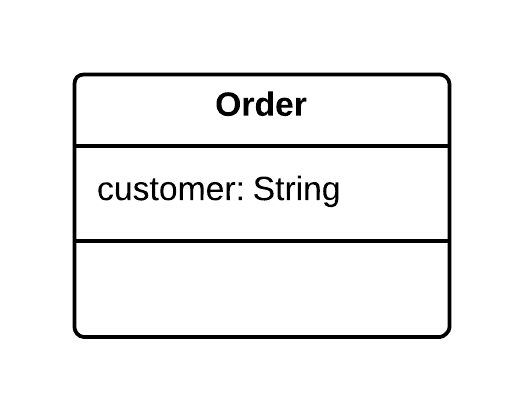
\includegraphics[scale=0.2]{replacedatavaluewithobjectproblem}
    \item \textbf{Solución} Cree una nueva clase, coloque el campo antiguo y su comportamiento en la clase y almacene el objeto de la clase en la clase original.\\
    \centering 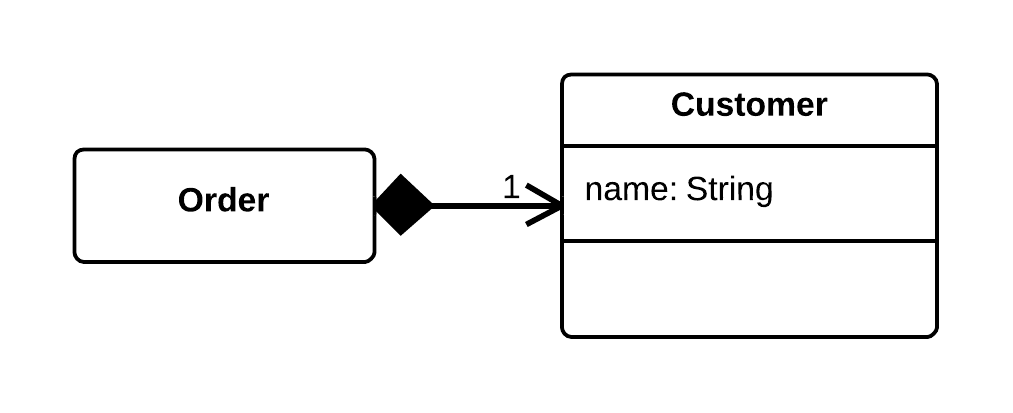
\includegraphics[scale=0.2]{replacedatavaluewithobjectsolution}
\end{itemize}
    
\subsection{Cambiar valor a referencia - Change Value to Reference}
\label{changevaluetoreference}
\begin{itemize}
    \item \textbf{Problema} Por lo tanto, tiene muchas instancias idénticas de una sola clase que necesita reemplazar con un solo objeto.\\
    \centering 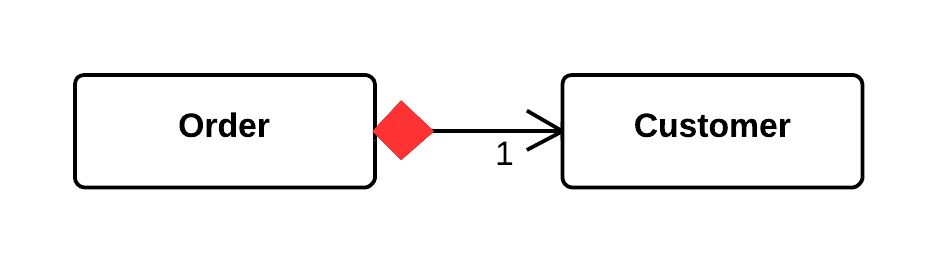
\includegraphics[scale=0.2]{changevaluetoreferenceproblem}
    \item \textbf{Solución} Convierta los objetos idénticos en un único objeto de referencia.\\
    \centering 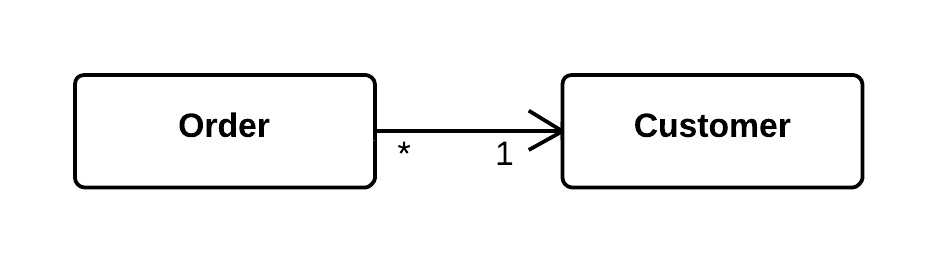
\includegraphics[scale=0.2]{changevaluetoreferencesolution}
\end{itemize}
    
\subsection{Cambiar valor a referencia - Change Reference to Value}
\label{changereferencetovalue}
\begin{itemize}
    \item \textbf{Problema} Tiene un objeto de referencia que es demasiado pequeño y se modifica con poca frecuencia para justificar la administración de su ciclo de vida.\\
    \centering 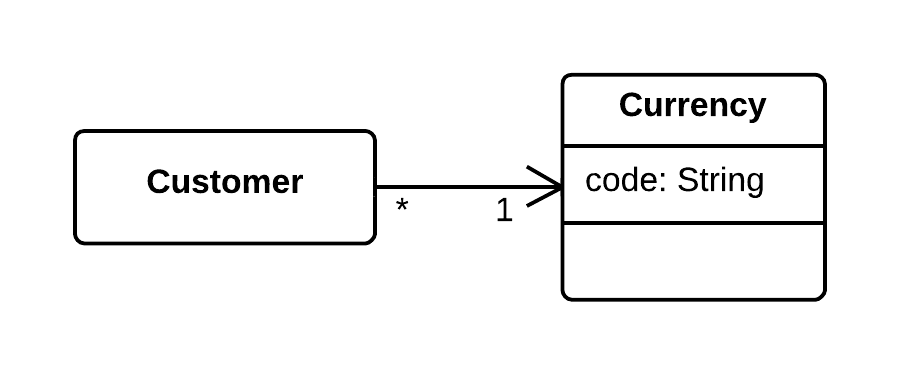
\includegraphics[scale=0.2]{changereferencetovalueproblem}
    \item \textbf{Solución} Conviértalo en un objeto de valor.\\
    \centering 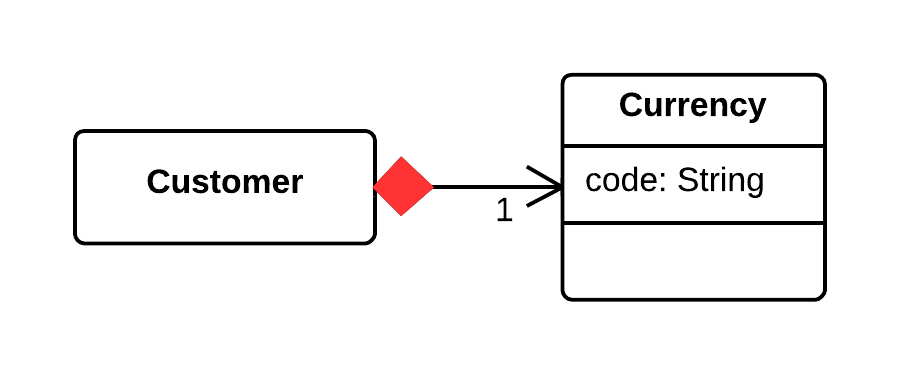
\includegraphics[scale=0.2]{changereferencetovaluesolution}
\end{itemize}
    
\subsection{Reemplazar matriz con objeto - Replace Array with Object}
\label{replacearraywithobject}
\begin{itemize}
    \item \textbf{Problema} Tiene una matriz que contiene varios tipos de datos.
    \lstinputlisting[language = java]{replacearraywithobjectproblem.java}
    \item \textbf{Solución} Reemplace la matriz con un objeto que tendrá campos separados para cada elemento.
    \lstinputlisting[language = java]{replacearraywithobjectsolution.java}
\end{itemize}
    
\subsection{Datos duplicados observados - Duplicate Observed Data}
\label{duplicateobserveddata}
\begin{itemize}
    \item \textbf{Problema} ¿Los datos de dominio se almacenan en clases responsables de la GUI?\\
    \centering 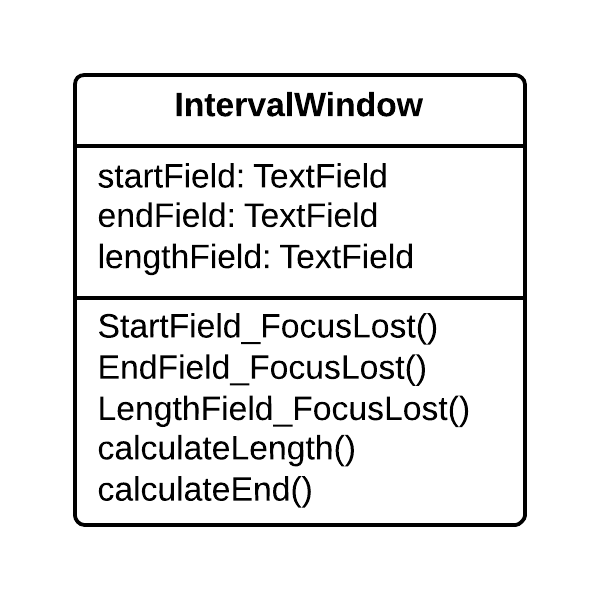
\includegraphics[scale=0.2]{duplicateobserveddataproblem}
    \item \textbf{Solución} Entonces es una buena idea separar los datos en clases separadas, asegurando la conexión y sincronización entre la clase de dominio y la GUI.\\
    \centering 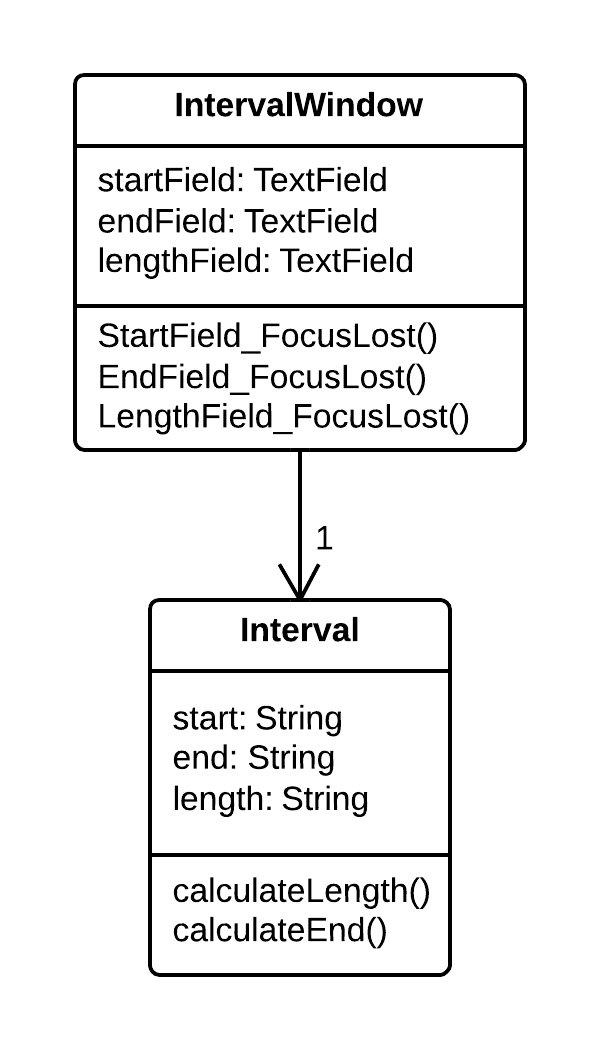
\includegraphics[scale=0.2]{duplicateobserveddatasolution}
\end{itemize}
    
\subsection{Cambiar asociación unidireccional a bidireccional - Change Unidirectional Association to Bidirectional}
\label{changeunidirectionalassociationtobidirectional}
\begin{itemize}
    \item \textbf{Problema} Tiene dos clases que cada una necesita para usar las características de la otra, pero la asociación entre ellas es solo unidireccional.\\
    \centering 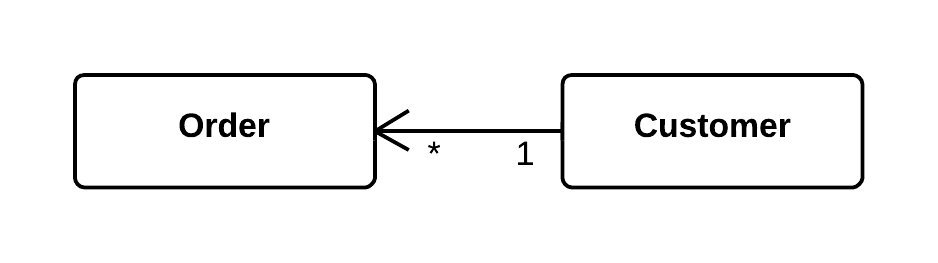
\includegraphics[scale=0.2]{changeunidirectionalassociationtobidirectionalproblem}
    \item \textbf{Solución} Agregue la asociación que falta a la clase que la necesita.\\
    \centering 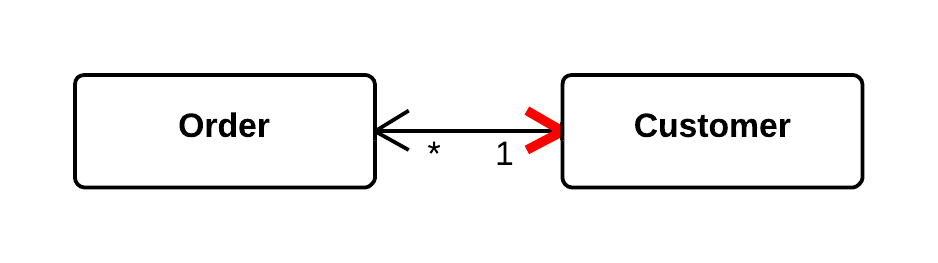
\includegraphics[scale=0.2]{changeunidirectionalassociationtobidirectionalsolution}
\end{itemize}
    
\subsection{Cambiar la asociación bidireccional a unidireccional - Change Bidirectional Association to Unidirectional}
\label{changebidirectionalassociationtounidirectional}
\begin{itemize}
    \item \textbf{Problema} Tiene una asociación bidireccional entre clases, pero una de las clases no usa las características de la otra.\\
    \centering 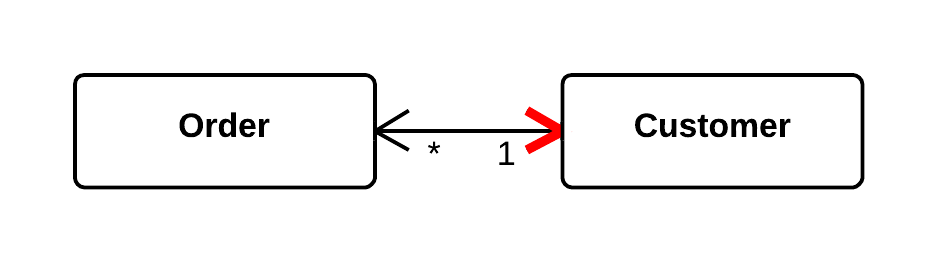
\includegraphics[scale=0.2]{changebidirectionalassociationtounidirectionalproblem}
    \item \textbf{Solución} Eliminar la asociación no utilizada.\\
    \centering 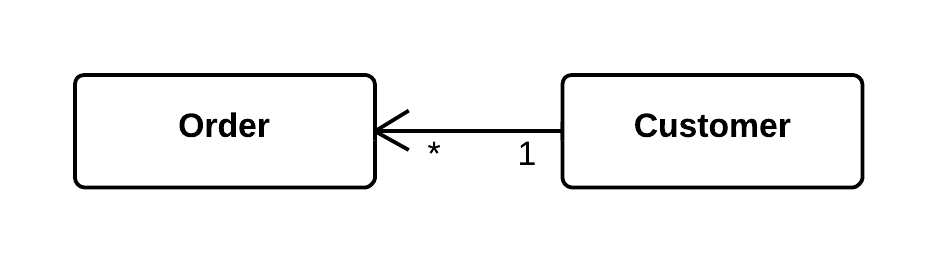
\includegraphics[scale=0.2]{changebidirectionalassociationtounidirectionalsolution}
\end{itemize}
    
\subsection{Reemplazar número mágico con constante simbólica - Replace Magic Number with Symbolic Constant}
\label{replacemagicnumberwithsymbolicconstant}
\begin{itemize}
    \item \textbf{Problema} Su código usa un número que tiene un cierto significado.
    \lstinputlisting[language = java]{replacemagicnumberwithsymbolicconstantproblem.java}
    \item \textbf{Solución} Reemplace este número con una constante que tenga un nombre legible por humanos que explique el significado del número.
    \lstinputlisting[language = java]{replacemagicnumberwithsymbolicconstantsolution.java}
\end{itemize}
    
\subsection{Campo encapsulado - Encapsulate Field}
\label{encapsulatefield}
\begin{itemize}
    \item \textbf{Problema} Tienes un campo público.
    \lstinputlisting[language = java]{encapsulatefieldproblem.java}
    \item \textbf{Solución} Haga que el campo sea privado y cree métodos de acceso para él.
    \lstinputlisting[language = java]{encapsulatefieldsolution.java}
\end{itemize}
    
\subsection{Colección encapsulada - Encapsulate Collection}
\label{encapsulatecollection}
\begin{itemize}
    \item \textbf{Problema} Una clase contiene un campo de colección y un getter y setter simple para trabajar con la colección.\\
    \centering 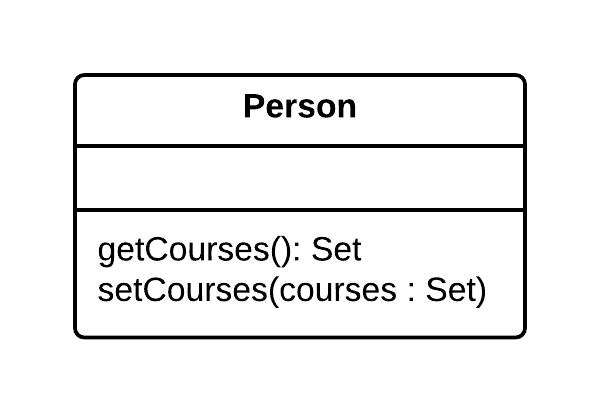
\includegraphics[scale=0.2]{encapsulatecollectionproblem}
    \item \textbf{Solución} Haga que el valor devuelto sea de solo lectura y cree métodos para agregar / eliminar elementos de la colección.\\
    \centering 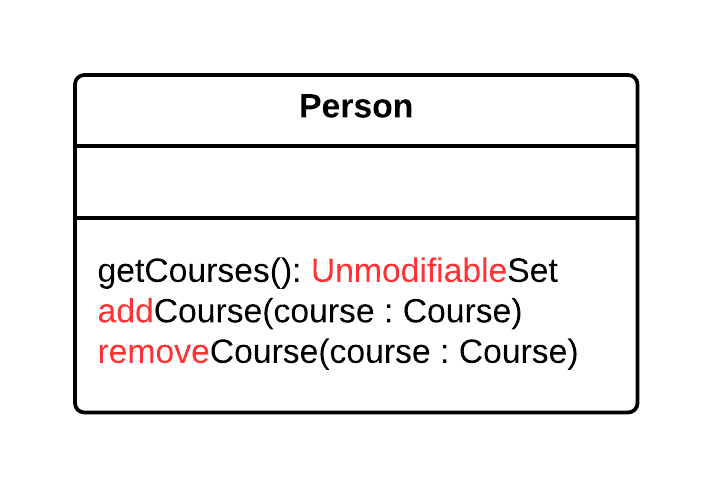
\includegraphics[scale=0.2]{encapsulatecollectionsolution}
\end{itemize}
    
\subsection{Reemplazar el tipo de dato con clase -  Replace Type Code with Class}
¿Qué es el tipo de dato? El tipo de dato ocurre cuando, en lugar de un tipo de datos separado, tiene un conjunto de números o cadenas que forman una lista de valores permitidos para alguna entidad. A menudo, estos números y cadenas específicos reciben nombres entendibles a través de constantes, razón por la cual se encuentra tanto tipo de dato .
\label{replacetypecodewithclass}
\begin{itemize}
    \item \textbf{Problema} Una clase tiene un campo que contiene un tipo de dato. Los valores de este tipo no se utilizan en condiciones de operador y no afectan el comportamiento del programa.\\
    \centering 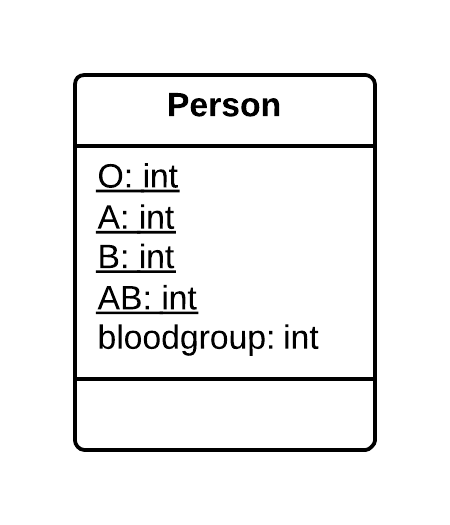
\includegraphics[scale=0.2]{replacetypecodewithclassproblem}
    \item \textbf{Solución} Cree una nueva clase y use sus objetos en lugar de los valores del tipo de dato.\\
    \centering 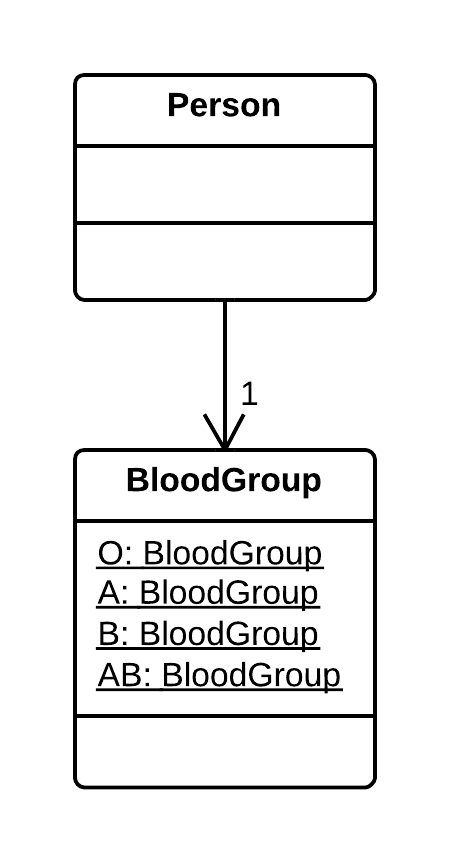
\includegraphics[scale=0.2]{replacetypecodewithclasssolution}
\end{itemize}
    
\subsection{Reemplazar el tipo de dato con subclases -  Replace Type Code with Subclasses}
¿Qué es el tipo de dato? El tipo de dato ocurre cuando, en lugar de un tipo de datos separado, tiene un conjunto de números o cadenas que forman una lista de valores permitidos para alguna entidad. A menudo, estos números y cadenas específicos reciben nombres entendibles a través de constantes, razón por la cual se encuentra tanto tipo de dato .
\label{replacetypecodewithsubclasses}
\begin{itemize}
    \item \textbf{Problema} Tiene un tipo codificado que afecta directamente el comportamiento del programa (los valores de este campo activan varios códigos en condicionales).\\
    \centering 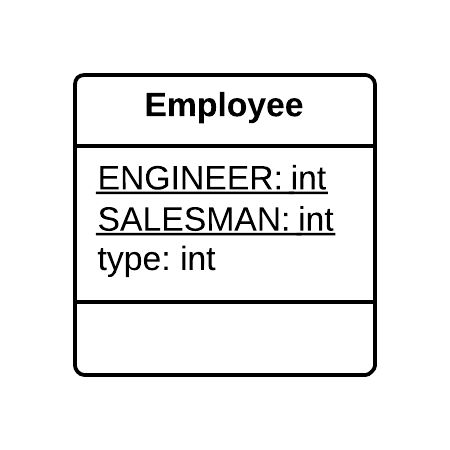
\includegraphics[scale=0.2]{replacetypecodewithsubclassesproblem}
    \item \textbf{Solución} Cree subclases para cada valor del tipo codificado. Luego extraiga los comportamientos relevantes de la clase original a estas subclases. Reemplace el código de flujo de control con polimorfismo.\\
    \centering 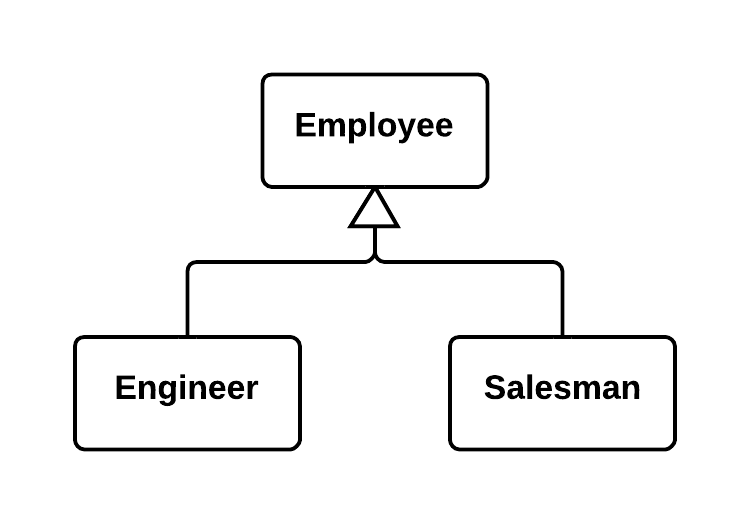
\includegraphics[scale=0.2]{replacetypecodewithsubclassessolution}
\end{itemize}
    
\subsection{Reemplazar el tipo de dato con estado / estrategia -  Replace Type Code with State/Strategy}
¿Qué es el tipo de dato? El tipo de dato ocurre cuando, en lugar de un tipo de datos separado, tiene un conjunto de números o cadenas que forman una lista de valores permitidos para alguna entidad. A menudo, estos números y cadenas específicos reciben nombres entendibles a través de constantes, razón por la cual se encuentra tanto tipo de dato .
\label{replacetypecodewithstatestrategy}
\begin{itemize}
    \item \textbf{Problema} Tiene un tipo codificado que afecta el comportamiento, pero no puede usar subclases para deshacerse de él.\\
    \centering 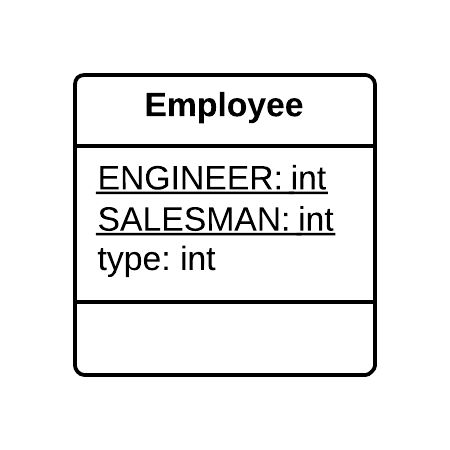
\includegraphics[scale=0.2]{replacetypecodewithstatestrategyproblem}
    \item \textbf{Solución} Reemplace el tipo de dato con un objeto de estado. Si es necesario reemplazar un valor de campo con el tipo de dato, otro objeto de estado se "conecta".\\
    \centering 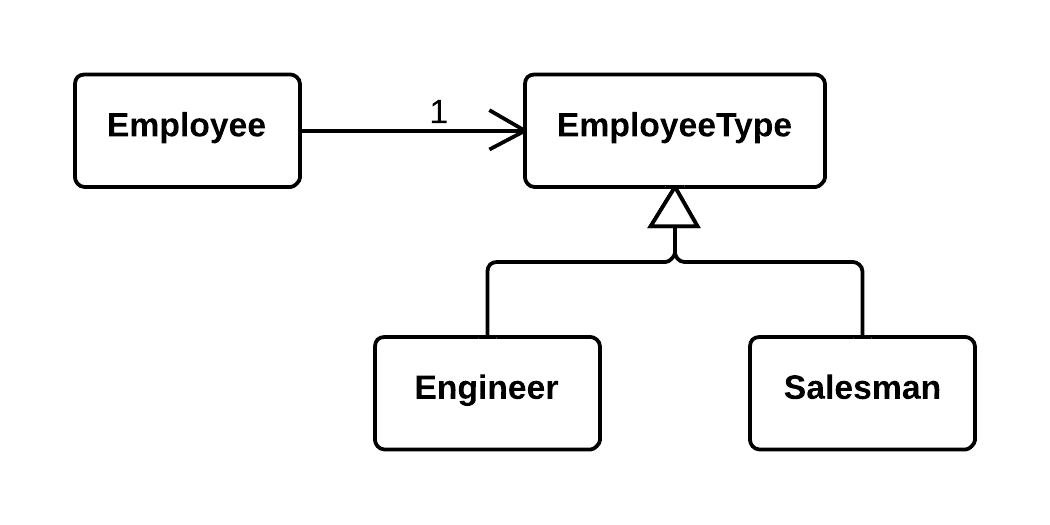
\includegraphics[scale=0.2]{replacetypecodewithstatestrategysolution}
\end{itemize}
    
\subsection{Reemplazar subclase con campos -  Replace Subclass with Fields}
\label{replacesubclasswithfields}
\begin{itemize}
    \item \textbf{Problema} Tiene subclases que difieren solo en sus métodos (de retorno constante).\\
    \centering 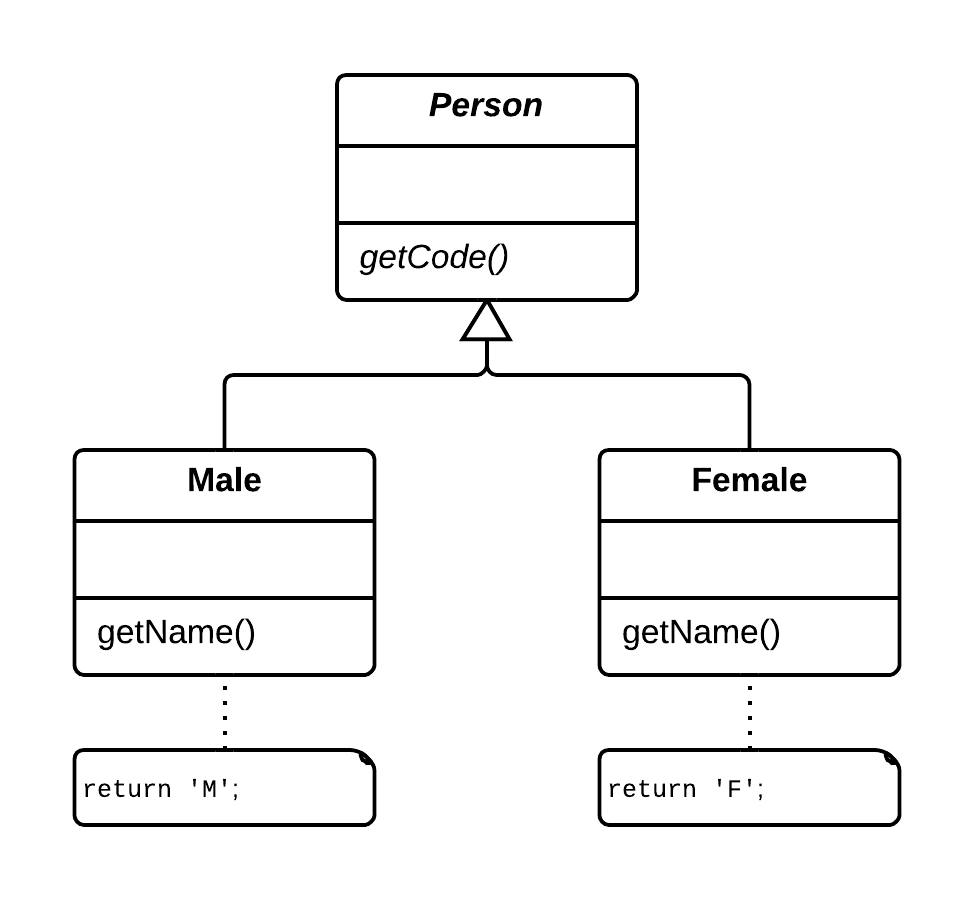
\includegraphics[scale=0.2]{replacesubclasswithfieldsproblem}
    \item \textbf{Solución} Reemplace los métodos con campos en la clase principal y elimine las subclases.\\
    \centering 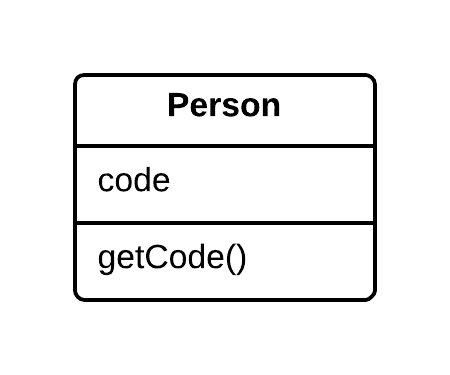
\includegraphics[scale=0.2]{replacesubclasswithfieldssolution}
\end{itemize}

%%%%%%%%% --- Fin - Cosmin --- %%%%%%%%%


\section{Simplificación de Expresiones Condicionales - Simplifying Conditional Expressions}

\label{renombrarmetodo}Los condicionales tienden a volverse más complicadas en su lógica a lo largo del tiempo, y también tenemos varias técnicas para resolver este tipo de problemas.

\subsection{Descomponer Condicionales - Decompose Conditional}  
\begin{itemize}
    \item \textbf{Problema} Tiene un condicional complejo (if-then / else o switch).
    
    \lstinputlisting[language = java]{descomposeConditionalProblem.java}
    
    \item \textbf{Solución} Descomponer las partes complejas del condicional en métodos separados: la condición, then y else.
    
    \lstinputlisting[language = java]{descomposeConditionalSolution.java}
\end{itemize}

\subsection{Consolidar la Expresión del Condicional - Consolidate Conditional Expression}  \begin{itemize}
    \item \textbf{Problema} Tiene múltiples condicionales que conducen al mismo resultado o acción.
    
    \lstinputlisting[language = java]{consolidateConditionalExpressionProblem.java}
    
    \item \textbf{Solución} Consolidar todos estos condicionales en una sola expresión.
    
    \lstinputlisting[language = java]{consolidateConditionalExpressionSolution.java}
\end{itemize}
    
\subsection{Consolidar Fragmentos Condicionales Duplicados - Consolidate Duplicate Conditional Fragments} 
\begin{itemize}
    \item \textbf{Problema} Se puede encontrar un código idéntico en todas las ramas de un condicional.
    
    \lstinputlisting[language = java]{consolidateDuplicateConditionalFragmentsProblem.java}
    
    \item \textbf{Solución} Mover el código fuera del condicional.
    
    \lstinputlisting[language = java]{consolidateDuplicateConditionalFragmentsSolution.java}
\end{itemize}
    
\subsection{Eliminar Indicador de Control - Remove Control Flag} 
 \begin{itemize}
    \item \textbf{Problema} Tiene una variable booleana que actúa como un indicador de control para múltiples expresiones booleanas.
    \item \textbf{Solución} En lugar de la variable, use break, continue y return.
\end{itemize}
    
\subsection{Reemplazar Condicionales Anidados con Cláusulas de Guardia - Replace Nested Conditional with Guard Clauses} 
\label{replaceNestedConditionalWithGuardClauses}
 \begin{itemize}
    \item \textbf{Problema} Tiene un grupo de condicionales anidados y es difícil determinar el flujo normal de ejecución del código.
    
    \lstinputlisting[language = java]{replaceNestedConditionalProblem.java}
    
    \item \textbf{Solución} Aislar todas las verificaciones especiales y casos extremos en cláusulas separadas y colocarlas antes de las verificaciones principales. Idealmente, debe tener una lista "plana" de condicionales, uno tras otro.
    
    \lstinputlisting[language = java]{replaceNestedConditionalSolution.java}
\end{itemize}
    
\subsection{Reemplazar Condicionales con Polimorfismo - Replace Conditional with Polymorphism}     
\begin{itemize}
    \item \textbf{Problema} Tiene un condicional que realiza varias acciones dependiendo del tipo de objeto o de las propiedades.
    
    \lstinputlisting[language = java]{replaceConditionalPolyProblem.java}
    
    \item \textbf{Solución} Crear subclases que coincidan con las ramas del condicional. En ellos, crear un método compartido y mover el código de la rama correspondiente del condicional. Luego reemplazar el condicional con la llamada al método relevante. El resultado es que la implementación adecuada se logrará a través del polimorfismo dependiendo de la clase de objeto.
    
    \lstinputlisting[language = java]{replaceConditionalPolySolution.java}
\end{itemize}
    
\subsection{Introducir Objetos Nulos - Introduce Null Object}        
\begin{itemize}
    \item \textbf{Problema} Dado que algunos métodos devuelven null en lugar de objetos reales, hay varias comprobaciones de null en el código.
    
    \lstinputlisting[language = java]{introduceNullObjectProblem.java}
    
    \item \textbf{Solución} En lugar de null, hacer que devuelva un objeto nulo que exhiba el comportamiento predeterminado.
    
    \lstinputlisting[language = java]{introduceNullObjectSolution.java}
\end{itemize}    

 \subsection{Introducir Aserciones - Introduce Assertion}    
\begin{itemize}
    \item \textbf{Problema} Para que una parte del código funcione correctamente, ciertas condiciones o valores deben ser verdaderos.
    
    \lstinputlisting[language = java]{introduceAssertionProblem.java}
    
    \item \textbf{Solución} Reemplazar estas suposiciones por comprobaciones de aserción específicos.
    
    \lstinputlisting[language = java]{introduceAssertionSolution.java}
\end{itemize}  

%%%%%%%%% ANTONIO MIGUEL %%%%%%%%%
\section{Método simplificado de llamadas}

Estas técnicas hacen que las llamadas a métodos sean más simples y fáciles de entender. Esto, a su vez, simplifica las interfaces para la interacción entre clases.

\subsection{Renombrar método - Rename Method}
\label{renamemethod}
\begin{itemize}
    \item \textbf{Problema} Aparece cuando un método no explica lo que hace 
    \item \textbf{Solución} Se renombra el método
\end{itemize}

\subsection{Añadir parámetro - Add Parameter}
\label{addparameter}
\begin{itemize}
    \item \textbf{Problema} Un método no tiene suficientes datos para realizar ciertas acciones.
    \item \textbf{Solución} Añada un nuevo parámetro para pasar los datos necesarios.
\end{itemize}
    
\subsection{Borrar parámetro - Remove Parameter}
\label{removeparameter}
\begin{itemize}
    \item \textbf{Problema} Un parámetro no se utiliza en el cuerpo de un método.
    \item \textbf{Solución} Elimina el parámetro.
\end{itemize}

\subsection{Consulta separada del modificador - Separate Query from Modifier}
\label{separatequeryfrommodifier}
\begin{itemize}
    \item \textbf{Problema} ¿Tiene un método que devuelve un valor pero también cambia algo dentro de un objeto?
    \item \textbf{Solucion} Divida el método en dos métodos separados. Como era de esperar, uno de ellos debería devolver el valor y el otro modifica el objeto.
\end{itemize}

\subsection{Método parametrizado - Parameterize Methodr}
\label{parameterizemethod}
\begin{itemize}
    \item \textbf{Problema} Múltiples métodos realizan acciones similares que son diferentes solo en sus valores internos, números u operaciones.
    \item \textbf{Solución} Combine estos métodos utilizando un parámetro que pasará el valor especial necesario.
\end{itemize}

\subsection{Reemplazar parametro con un método explicito - Replace Parameter with Explicit Methods}
\label{replaceparameterwithexplicitmethods}
\begin{itemize}
    \item \textbf{Problema} Un método se divide en partes, cada una de las cuales se ejecuta según el valor de un parámetro.
    \item \textbf{Solución} Extraiga las partes individuales del método en sus propios métodos y llámelas en lugar del método original.
\end{itemize}

\subsection{Preserva todo el objeto - Preserve Whole Object}
\label{preservewholeobject}
\begin{itemize}
    \item \textbf{Problema} Obtiene varios valores de un objeto y luego los pasa como parámetros a un método.
    \item \textbf{Solución} en su lugar, intente pasar todo el objeto.
\end{itemize}
    
\lstinputlisting[language = java]{preserveWholeObject.java}

\subsection{Reemplazar parámetro con llamada a método - Replace Parameter with Method Call}
\label{replaceparameterwithmethodcall}
\begin{itemize}
    \item \textbf{Problema} Antes de la llamada a un método, se ejecuta un segundo método y su resultado se envía de vuelta al primer método como argumento. Pero el valor del parámetro podría haberse obtenido dentro del método que se llama.
    \item \textbf{Solución} En lugar de pasar el valor a través de un parámetro, coloque el código de obtención de valor dentro del método.
\end{itemize}

\lstinputlisting[language = java]{replaceParameterWithMethodCall.java}

\subsection{Introducir un objeto como parámetro - Introduce Parameter Object}
\label{introduceparameterobject}
\begin{itemize}
    \item \textbf{Problema} Sus métodos contienen un grupo repetitivo de parámetros.   
   \item \textbf{Solución} Reemplace estos parámetros con un objeto.
\end{itemize}

\subsection{Eliminar método de configuración - Remove Setting Method}
\label{removesettingmethod}
\begin{itemize}
    \item \textbf{Problema} El valor de un campo debe establecerse solo cuando se crea, y no cambiar en ningún momento después de eso.
    \item \textbf{Solución}  Elimine los métodos que establecen el valor del campo.
\end{itemize}

\subsection{Método oculto - Hide Method}
\label{hidemethod}
\begin{itemize}
    \item \textbf{Problema} Otras clases no usan un método o solo se usan dentro de su propia jerarquía de clases.
    \item \textbf{Solución} Haz el método privado o protegido.
\end{itemize}

\subsection{Reemplazar constructor con método factory - Replace Constructor with Factory Method}
\label{replaceconstructorwithfactorymethod}
\begin{itemize}
    \item \textbf{Problema} Tiene un constructor complejo que hace algo más que simplemente establecer valores de parámetros en campos de objeto.
    \item \textbf{Solución} Cree un método factory y usalo para reemplazar las llamadas al  constructor.
\end{itemize}
    
\lstinputlisting[language = java]{replaceConstructorWithFactoryMethod.java}

\subsection{Reemplazar código de error con excepción - Replace Error Code with Exception}
\label{replaceerrorcodewithexception}
\begin{itemize}
    \item \textbf{Problema} ¿Un método devuelve un valor especial que indica un error?
    \item \textbf{Solución} Devolver una excepción.
\end{itemize}
    
\lstinputlisting[language = java]{replaceErrorCodeWithException.java}

\subsection{Reemplazar excepción con test - Replace Exception with Test}
\label{replaceexceptionwithtest}
\begin{itemize}
    \item \textbf{Problema} ¿Lanzas una excepción en un lugar donde una simple prueba haría el trabajo?
    \item \textbf{Solución} Reemplace la excepción con una prueba de condición.
\end{itemize}
    
\lstinputlisting[language = java]{replaceExceptionWithTest.java}

%%%%% Dealing with Generalisation

\section{Tratando con la generalización - Dealing with Generalisation}

La abstracción tiene su propio grupo de técnicas de refactorización, principalmente asociadas con la funcionalidad de movimiento a lo largo de la jerarquía de herencia de clases, creando nuevas clases e interfaces, y reemplazando la herencia con delegación y viceversa.

\subsection{Campo Pull Up - Pull Up Field}
\label{pullupfield}
\begin{itemize}
    \item \textbf{Problema} Dos clases tienen el mismo campo.
    \item \textbf{Solución} Elimine el campo de las subclases y muévalo a la superclase.
\end{itemize}

\subsection{Método Pull Up - Pull Up Method}
\label{pullupmethod}
\begin{itemize}
    \item \textbf{Problema} sus subclases tienen métodos que realizan un trabajo similar.
    \item \textbf{Solución} Haga que los métodos sean idénticos y luego muévalos a la superclase relevante
\end{itemize}

\subsection{Levante el cuerpo del constructor - Pull Up Constructor Body}
\label{pullupconstructorbody}
\begin{itemize}
    \item \textbf{Problema} Sus subclases tienen constructores con código que es casi idéntico.
    \item \textbf{Solución} Cree un constructor de superclase y mueva el código que es el mismo en las subclases. Llame al constructor de la superclase en los constructores de la subclase.
\end{itemize}
\lstinputlisting[language = java]{pullUpConstructorBody.java}

\subsection{Método de empuje - Push Down Method}
\label{pushdownmethod}
\begin{itemize}
    \item \textbf{Problema} ¿El comportamiento implementado en una superclase solo lo usan una (o algunas) subclases?
    \item \textbf{Solución} Mueva este comportamiento a las subclases.
\end{itemize}

\subsection{Campo de empuje – Push down field}
\label{pushdownfield}
\begin{itemize}
    \item \textbf{Problema} ¿Se utiliza un campo solo en algunas subclases?
    \item \textbf{Solución} Mueva el campo a estas subclases.
\end{itemize}

\subsection{Extraer subclase - Extract Subclass}
\label{extractsubclass}
\begin{itemize}
    \item \textbf{Problema} Una clase tiene características que se usan solo en ciertos casos.
    \item \textbf{Solución} Cree una subclase y úsela en estos casos.
\end{itemize}

\subsection{Extraer superclase - Extract Superclass}
\label{extractsuperclass}
\begin{itemize}
    \item \textbf{Problema} Tiene dos clases con campos y métodos comunes.
    \item \textbf{Solución} Cree una superclase compartida para ellos y muévales todos los campos y métodos idénticos.
\end{itemize}

\subsection{Interfaz de extracción - Extract Interface}
\label{extractinterface}
\begin{itemize}
    \item \textbf{Problema} Varios clientes utilizan la misma parte de una interfaz de clase. Otro caso: parte de la interfaz en dos clases es la misma.
    \item \textbf{Solución} Mueva esta porción idéntica a su propia interfaz.
\end{itemize}

\subsection{Contraer jerarquía - Collapse Hierarchy}
\label{colapsehierarchy}
\begin{itemize}
    \item \textbf{Problema} Tiene una jerarquía de clases en la que una subclase es prácticamente igual a su superclase.
    \item \textbf{Solución} Fusionar la subclase y la superclase.
\end{itemize}

\subsection{Método de plantilla de formulario - Form Template Method}
\label{formtemplatemethod}
\begin{itemize}
    \item \textbf{Problema} Sus subclases implementan algoritmos que contienen pasos similares en el mismo orden.
    \item \textbf{Solución}  Mueva la estructura del algoritmo y los pasos idénticos a una superclase, y deje la implementación de los diferentes pasos en las subclases.
\end{itemize}

\subsection{Reemplazar herencia con delegación- Replace Inheritance with Delegation}
\label{replaceinheritancewithdelegation}
\begin{itemize}
    \item \textbf{Problema} Tiene una subclase que usa solo una parte de los métodos de su superclase (o no es posible heredar los datos de la superclase).
    \item \textbf{Solución} Cree un campo y coloque un objeto de superclase en él, delegue métodos al objeto de superclase y elimine la herencia.
\end{itemize}

\subsection{Reemplazar delegación con herencia - Replace Delegation with Inheritance}
\label{replacedelegationwithinheritance}
\begin{itemize}
    \item \textbf{Problema} Una clase contiene muchos métodos simples que delegan a todos los métodos de otra clase.
    \item \textbf{Solución} Haga de la clase un heredero delegado, lo que hace innecesarios los métodos de delegación.
\end{itemize}

%%%%%%%%%%%%%%%%%%%%%%%%%%%%%%%%%%%%

\section{Otras refactorizaciones de Fowler}
% https://refactoring.com/catalog/
\subsection{Grupo 1}
Change Function Declaration

Change Signature 

Inline Function

Inline Variable

Introduce Explaining Variable

Introduce Special Case

Move Function

Move Statements into Function

Move Statements to Callers

%%%%%%%%%%%%%%%%%%%%%%%%%-Alejandro-%%%%%%%%%%%%%%%%%%%%%%%%%%%%%%

\subsection{Grupo 2}
\textbf{Parameterize Function}
\label{ParameterizeFunction}
\begin{itemize}
    \item \textbf{Problema} Múltiples métodos llevan a cabo acciones similares que son distintos solo en sus valores internos, números u operaciones.
    \lstinputlisting[language = java]{parameterizeFunctionProblem.java}
    
    \item \textbf{Solución} Combina estos métodos usando un parámetro que pasará el valor necesitado.
      \lstinputlisting[language = java]{parameterizeFunctionSolution.java}
\end{itemize}

\textbf{Remove Flag Argument}
\label{RemoveFlagArgument}
\begin{itemize}
    \item \textbf{Problema} Un método que cambia los valores de distintas variables en función de varios \textit{if}.
    \lstinputlisting[language = java]{removeFlagArgumentProblem.java}
    \item \textbf{Solución} Partir el método a método por \textit{if}.
    \lstinputlisting[language = java]{removeFlagArgumentSolution.java}
\end{itemize}


\textbf{Remove Subclass}
\label{RemobeSubclass}
\begin{itemize}
    \item \textbf{Problema} Tienes subclases que difieren solo en sus métodos que devuelven constantes.
    \lstinputlisting[language = java]{removeSubclassProblem.java}
    \item \textbf{Solución} Reemplaza los métodos con campos en la clase padre y borra las subclases.
    \lstinputlisting[language = java]{removeSubclassSolution.java}
\end{itemize}

\textbf{Remove Field}
\label{RenameField}
\begin{itemize}
    \item \textbf{Problema} El nombre del campo no revela correctamente su propósito.
    \lstinputlisting[language = java]{renameFieldProblem.java}
    \item \textbf{Solución} Se cambia el campo por un nombre más adecuado.
    \lstinputlisting[language = java]{renameFieldSolution.java}
\end{itemize}

\textbf{Rename Function}
\label{RenameFunction}
\begin{itemize}
    \item \textbf{Problema} El nombre de un método no explica que hace.
    \lstinputlisting[language = java]{renameFunctionProblem.java}
    \item \textbf{Solución} Renombrar el método.
    \lstinputlisting[language = java]{renameFunctionSolution.java}
\end{itemize}

\textbf{Rename Variable}
\label{RenameVariable}
\begin{itemize}
    \item \textbf{Problema} El nombre de la variable no es explicativo.
    \lstinputlisting[language = java]{renameVariableProblem.java}
    \item \textbf{Solución} Cambiar el nombre por uno más explicativo.
    \lstinputlisting[language = java]{renameVariableSolution.java}
\end{itemize}

\textbf{Replace Command with Function}
\label{ReplaceCommandWithFunction}
\begin{itemize}
    \item \textbf{Problema} Se crea una clase para llevar a cabo una función.
    \lstinputlisting[language = java]{replaceCommandWithFunctionProblem.java}
    \item \textbf{Solución} Eliminar esta clase e incluirla como función en otra clase.
    \lstinputlisting[language = java]{replaceCommandWithFunctionSolution.java}
\end{itemize}

%%%%%%%%%%%%%%%%%%%%%%%%%%%%%%%%%%%%%%%%%%%%%%%%%%%%%%%%%%%%%%%%%%%%%%

\subsection{Grupo 3}
Replace Constructor with Factory Method

Replace Control Flag with Break

Replace Derived Variable with Query

Replace Exception with Precheck

Replace Function with Command

Replace Inline Code with Function Call

\subsection{Grupo 4}
\textbf{Replace Loop with Pipeline}
\label{ReplaceLoopWithPipeline}
\begin{itemize}
    \item \textbf{Problema} Usar un bucle para listar un conjunto de objetos en vez de usar una librería de tuberías.
    \lstinputlisting[language = java]{ReplaceLoopWithPipelineProblem.java}
    
    \item \textbf{Solución} Cambiar el bucle por un método de la librería de tuberías.
    \lstinputlisting[language = java]{ReplaceLoopWithPipelineSolution.java}
\end{itemize}

\textbf{Replace Magic Literal}
\label{ReplaceMagicLiteral}
\begin{itemize}
    \item \textbf{Problema} Usar un número sin identificar para representar una constante matemática.
    \lstinputlisting[language = java]{ReplaceMagicLiteralProblem.java}
    
    \item \textbf{Solución} Cambiar el número por una constante con un nombre repesentativo.
    \lstinputlisting[language = java]{ReplaceMagicLiteralSolution.java}
\end{itemize}

\textbf{Replace Parameter with Query}
\label{ReplaceParameterWithQuery}
\begin{itemize}
    \item \textbf{Problema} Incluir atributos innecesarios en un método.
    \lstinputlisting[language = java]{ReplaceParameterWithQueryProblem.java}
    
    \item \textbf{Solución} Simplificar estos atributos accediendo a estos desde el método.
    \lstinputlisting[language = java]{ReplaceParameterWithQuerySolution.java}
\end{itemize}

\textbf{Replace Primitive with Object}
\label{ReplacePrimitiveWithObject}
\begin{itemize}
    \item \textbf{Problema} Usar demasiados valores primitivos en una sentencia.
    \lstinputlisting[language = java]{ReplacePrimitiveWithObjectProblem.java}
    
    \item \textbf{Solución} Convertir estos valores primitivos en objetos.
    \lstinputlisting[language = java]{ReplacePrimitiveWithObjectSolution.java}
\end{itemize}

\textbf{Replace Query with Parameter}
\label{replaceQueryWithParameter}
\begin{itemize}
    \item \textbf{Problema} Justamente lo contrario a \ref{ReplaceParameterWithQuery}
    \lstinputlisting[language = java]{ReplacePrimitiveWithObjectProblem.java}
    
    \item \textbf{Solución} Justamente lo contrario a \ref{ReplaceParameterWithQuery}
    \lstinputlisting[language = java]{ReplacePrimitiveWithObjectSolution.java}
\end{itemize}

\textbf{Replace Record with Data Class}
\label{ReplaceRecordWithDataClass}
\begin{itemize}
    \item \textbf{Problema} Tener demasiados valores para un dato de diccionario.
    \lstinputlisting[language = java]{EncapsulateRecordProblem.java}
    
    \item \textbf{Solución} Transformar este valor en una clase.
    \lstinputlisting[language = java]{EncapsulateRecordSolution.java}
\end{itemize}

\textbf{Replace Subclass with Delegate}
\label{ReplaceSubclassWithDelegate}
\begin{itemize}
    \item \textbf{Problema} Tienes una clase que usar porciones de métodos de su superclase.
    \lstinputlisting[language = java]{EncapsulateRecordProblem.java}
    
    \item \textbf{Solución} Crear un capto y poner un objeto superclase en este, métodos delegados al objeto de la superclase y deshacerse de la herencia.
    \lstinputlisting[language = java]{EncapsulateRecordSolution.java}
\end{itemize}


\subsection{Grupo 5}
Replace Superclass with Delegate
\label{replaceSuperclassWithDelegate}
\begin{itemize}
    \item \textbf{Problema} 
\end{itemize}

Replace Type Code with Class

Return Modified Value

Slide Statements

Split Loop

Split Phase

Split Variable



\chapter*{Correspondencia entre refactorizaciones}

\begin{longtable}{|p{200pt}|p{200pt}|}
\footnotesize
 Categoría Fowler &Categoría refactorización\\ 
\hline
    Add Parameter & Add Parameter\\ 
    Change Bidirectional Association to Unidirectional & \\ 
    Change Reference to Value & Change Reference to Value\\ 
    Change Unidirectional Association to Bidirectional & \\ 
    Change Value to Reference & Change Value to Reference\\ 
    Collapse Hierarchy & Collapse Hierarchy\\ 
 & Combine Functions into Class\\ 
 & Combine Functions into Transform\\ 
    Consolidate Conditional Expression & Consolidate Conditional Expression\\ 
    Consolidate Duplicate Conditional Fragments & Consolidate Duplicate Conditional Fragments\\ 
    Decompose Conditional & Decompose Conditional\\ 
    Duplicate Observed Data & \\ 
    Encapsulate Collection & Encapsulate Collection\\ 
    Encapsulate Field & Encapsulate Field \\ 
 & Encapsulate Record\\ 
 & Encapsulate Variable\\ 
    Extract Class & Extract Class\\ 
    Extract Interface & Extract Function\\ 
    Extract Method & Extract Method\\ 
    Extract Subclass & Extract Subclass \\ 
    Extract Superclass & Extract Superclass\\ 
    Extract Variable & Extract Variable\\ 
    Form Template Method & \\ 
    Hide Delegate & Hide Delegate\\ 
    Hide Method & \\ 
    Inline Class & Inline Class\\ 
    Inline Method & Inline Method\\ 
    Inline Temp & Inline Temp\\ 
    Introduce Assertion & Introduce Assertion\\ 
    Introduce Foreign Method & \\ 
    Introduce Local Extension & \\ 
    Introduce Null Object & Introduce Null Object\\ 
    Introduce Parameter Object & Introduce Parameter Object\\ 
    Move Field & Move Field\\ 
    Move Method & Move Method\\ 
    Parameterize Method & Parameterize Method\\ 
    Preserve Whole Object & Preserve Whole Object\\ 
    Pull Up Constructor Body & Pull Up Constructor Body\\ 
    Pull Up Field & Pull Up Field\\ 
    Pull Up Method & Pull Up Method\\ 
    Push Down Field & Push Down Field\\ 
    Push Down Method & Push Down Method\\ 
    Remove Assignments to Parameters & Remove Assignments to Parameters \\ 
    Remove Control Flag & Remove Control Flag\\ 
    Remove Middle Man & Remove Middle Man\\ 
    Remove Parameter & Remove Parameter \\ 
    Remove Setting Method & Remove Setting Method\\ 
    Rename Method & Rename Method\\ 
    Replace Array with Object & \\ 
    Replace Conditional with Polymorphism & Replace Conditional with Polymorphism\\ 
    Replace Constructor with Factory Method & Replace Constructor with Factory Function\\ 
    Replace Data Value with Object & Replace Data Value with Object\\ 
    Replace Delegation with Inheritance & \\ 
    Replace Error Code with Exception & Replace Error Code with Exception\\ 
    Replace Exception with Test & Replace Exception with Test\\ 
    Replace Inheritance with Delegation & Replace Inheritance with Delegation\\ 
    Replace Magic Number with Symbolic Constant & Replace Magic Number with Symbolic Constant\\ 
    Replace Method with Method Object & Replace Method with Method Object\\ 
    Replace Nested Conditional with Guard Clauses & Replace Nested Conditional with Guard Clauses\\ 
    Replace Parameter with Explicit Methods & Replace Parameter with Explicit Methods\\ 
    Replace Parameter with Method Call & Replace Parameter with Method\\ 
    Replace Subclass with Fields & Replace Subclass with Fields\\ 
    Replace Temp with Query & Replace Temp with Query\\ 
    Replace Type Code with Class & \\ 
    Replace Type Code with State/Strategy & Replace Type Code with State/Strategy\\ 
    Replace Type Code with Subclasses & Replace Type Code with Subclasses\\ 
    Self Encapsulate Field & Self-Encapsulate Field\\ 
    Separate Query from Modifier & Separate Query from Modifier\\ 
    Split Temporary Variable & Split Temp\\ 
    Substitute Algorithm &     Substitute Algorithm\\
\end{longtable}





\chapter{Caso 1: Juan Soler}
 \textbf{Refactorizado por:} Jose Antonio Parra Sánchez \newline

\textbf{Propuestas: } Revisando el código, se puede apreciar una buena gestión de las clases ya que podemos encontrar una carpeta ``models'' que contiene los objetos que forman parte de la solución del problema. Pero, personalmente, dichos objetos no los habría colocado en un package distinto al del main. Otro package que podemos encontrar es ``util'', pero este solo tiene una clase vacía por lo que no sabría exactamente cual es su función. A continuación se señalarán algunas propuestas más enfocadas en el código.

\begin{itemize}
    \item \textbf{Comentarios: } En la clase main podemos encontrar un segmento de código comentado prescindible.
    \lstinputlisting[language = java, firstline=24,lastline=32]{alumno7MetodoLargo.java}
    
     \item \textbf{Renombrar Variable: } Siguiendo en la misma clase, hay una variable temporal que recibe el nombre de ``temp'', pero desde mi punto de vista puede resultar un nombre confuso por lo que yo lo reemplazaría por ``aux''.
     \lstinputlisting[language = java]{alumno7RenombrarVariable.java}
     
      \item \textbf{Método Largo: } El método ``introducirDatos()'' realiza más funciones de lo que su nombre indica, podría renombrarse el método a un nombre más adecuado o dividir el método en dos.
          \lstinputlisting[language = java]{alumno7MetodoLargo.java}
  
\end{itemize}

\chapter{Caso 2: Alejandro Francisco}
\textbf{Refactorizado por:} Juan Soler Márquez \newline

    \hyperref[longmethod]{\textbf{Long Method}}
      \newline

     \textbf{Razón:} El método es demasiado largo, realizando funciones distintas que podrían extraerse a métodos más pequeños.
    \newline
 \lstinputlisting[language = java]{case2AnalizarArchivoMethod.java}      \newline

 \hyperref[extractmethod]{\textbf{Extract Method}}
\newline
  \textbf{Razón:} Tiene métodos que no tienen nada que ver con la clase main, podrían extraerse a una subclase.
  \newline

  \lstinputlisting[language = java]{Case2Main.java} 
  
\newline

   \hyperref[replaceNestedConditionalWithGuardClauses]{\textbf{\textbf{Reemplazar condicionales anidados con clausulas de guardia}}}
   \newline

   \textbf{Razón:} Tiene demasiados condicionales anidados y es difícil determinar el flujo normal de ejecución del código. Solución aislar todas las verificaciones especiales y casos extremos en cláusulas separadas y colocarlas antes de las verificaciones principales. Idealmente, debe tener una lista "plana"de condicionales, uno tras otro.
   
   

   \newline

  \lstinputlisting[language = java]{Case2Main.java} 

\chapter {Caso 3: Francisco José Martín}
 \textbf{Refactorizado por:} Alejandro Francisco García Uclés \newline

    \hyperref[deadcode]{\textbf{Dead Code}}
    
    \textbf{Razón:} El constructor de la clase Pueblo que recibe una lista de tramos no se usa nunca.
    
    \lstinputlisting[language = java]{alumno2DeadCode.java}
    
    \hyperref[longmethod]{\textbf{Long Method}}
    
    \textbf{Razón:} El método contiene más de diez lineas, habiendo algunas que podrían sacarse a otros métodos. Como veremos más adelante.
    
    \lstinputlisting[language = java]{alumno2LongMethod.java}
    
    \hyperref[renamevariable]{\textbf{Rename Variable}}
    
    \textbf{Razón:} La variable no explica qué se quiere confirmar si es verdadero o falso.
    
    \lstinputlisting[language = java]{alumno2RenameVariable.java}
    
    \hyperref[renamefield]{\textbf{Rename Field}}
    
    \textbf{Razón:} El nombre del método, aunque bastante indicativo de lo que hace, podría serlo más.
    
    \lstinputlisting[language = java]{alumno2RenameField.java}
    
    \hyperref[extractmethod]{\textbf{Extract Method}}
    
    \textbf{Razón:} Del método MCD antes comentado en \textbf{LongMethod}, este condicional que da valor a una variable podría extraerse para un nuevo método.
    
    \lstinputlisting[language = java, firstline=10,lastline=14]{alumno2LongMethod.java}
    
    


\chapter {Caso 4: Francisco Jesús García López}
\textbf{Refactorizador:} Francisco José Martín







\chapter {Caso 5: Adalid Abraham Villanueva Hermoza}
\textbf{Refactoriza:} Fco Jesus Garcia López


\chapter {Caso 6: Marius Cosmin Magurean}
% refactorizado por: Adalid Abraham Villanueva Hermoza

\chapter {Caso 7: Jose Antonio Parra Sánchez}
\textbf{Refactoriza:} Antonio Miguel

Vamos a comenzar comentando por archivos.
Empezamos por \emph{Algorit.java}:

\lstinputlisting[language = java]{caso7Algorit.java}

Como podemos apreciar, en primer lugar, lo primero que debemos cambiar es el nombre del método, no solo porque los métodos públicos deben ir en mayúsculas, si no por que el método no explica bien lo que hace: \textbf{Rename Method (\ref{renamemethod})}

\newline
Mas modificaciones que podemos aplicar:

\begin{itemize}
    \item \textbf{Temp en línea} (\ref{inlinetemp}):
    \begin{itemize}
        \item Línea 10.
    \end{itemize}
    
    \item \textbf{Código muerto} (\ref{deadcode}):
    \begin{itemize}
        \item Línea 16.
        \item Línea 17.
        \item Línea 19.
        \item Línea 28.
        \item Línea 29.
        \item Línea 31.
        \item Línea 35.
    \end{itemize}
    
    \item \textbf{Renombrar variables} (\ref{RenameVariable}):
    \begin{itemize}
        \item Línea 7.
    \end{itemize}
    
    \item \textbf{Reemplazar condicionales anidados con clausulas de guardia} (\ref{replaceNestedConditionalWithGuardClauses}):
    \begin{itemize}
        \item Línea 11.
    \end{itemize}
    
    \item \textbf{Introducir un objeto como parámetro} (\ref{introduceparameterobject}):
    \begin{itemize}
        \item Línea 5.
    \end{itemize}
\end{itemize}

Continuamos con el archivo \textbf{Data.java}. Al igual que en el anterior archivo, lo primero que podemos observar es que los métodos públicos no están escritos con mayúsculas: \textbf{Rename Method (\ref{renamemethod})}.

\lstinputlisting[language = java]{caso7Data.java}

\text{Continuamos con más modificaciones}:
\begin{itemize}
    \item \textbf{Renombrar variables} (\ref{RenameVariable}):
    \begin{itemize}
        \item Línea 13.
    \end{itemize}
    
    \item \textbf{Añadir parámetro} (\ref{addparameter}):
    \begin{itemize}
        \item Línea 9. (Pasar el texto como parámetro para poder reutilizarlo.
    \end{itemize}
    
    \item \textbf{Añadir comprobación de errores}:
    \begin{itemize}
        \item Línea 19.
    \end{itemize}
\end{itemize}

Archivo \textbf{Table.java}:

\lstinputlisting[language = java]{caso7Table.java}
Al igual que el resto, métodos públicos con mayúsculas.

Archivo \textbf{Main.java}:
\lstinputlisting[language = java]{caso7Main.java}

\textbf{Refactorización}:
\begin{itemize}
    \item \textbf{Crear objetos}: Crear objetos para almacenar y ofrecer los resultados, haciendo más fácil administrar los campos.
\end{itemize}



\chapter {Caso 9: Antonio}
\textbf{Refactoriza:} Marius Cosmin Magurean\\

El Archivo \textbf{main.go} es donde se inicializán todos los valores y está el metodo main.
El cual tiene demasiadas lineas por tanto se debe analizar como un
\textbf{Método Largo (\ref{metodolargo})}.
\lstinputlisting[language = java]{caso9main.java}


\end{document}

